\documentclass[a4paper]{article}
\usepackage[ngerman]{babel}
\usepackage[utf8]{inputenc}
\usepackage{multicol}
\usepackage{calc}
\usepackage{ifthen}
\usepackage[landscape]{geometry}
\usepackage{amsmath,amsthm,amsfonts,amssymb}
\usepackage{color,graphicx,overpic}
\usepackage{xcolor, listings}
\usepackage[compact]{titlesec} %less space for headers
\usepackage{mdwlist} %less space for lists
\usepackage{pdflscape}
\usepackage{verbatim}
\usepackage[most]{tcolorbox}
\usepackage[hidelinks,pdfencoding=auto]{hyperref}
\usepackage{fancyhdr}
\usepackage{lastpage}
\pagestyle{fancy}
\fancyhf{}
\fancyhead[L]{Systemsicherheit}
\fancyfoot[L]{\thepage/\pageref{LastPage}}
\renewcommand{\headrulewidth}{0pt} %obere Trennlinie
\renewcommand{\footrulewidth}{0pt} %untere Trennlinie

\pdfinfo{
  /Title (Systemsicherheit - Cheatsheet)
  /Creator (TeX)
  /Producer (pdfTeX 1.40.0)
  /Author (Robert Jeutter)
  /Subject ()
}

%%% Code Listings
\definecolor{codegreen}{rgb}{0,0.6,0}
\definecolor{codegray}{rgb}{0.5,0.5,0.5}
\definecolor{codepurple}{rgb}{0.58,0,0.82}
\definecolor{backcolour}{rgb}{0.95,0.95,0.92}
\lstdefinestyle{mystyle}{
 backgroundcolor=\color{backcolour},  
 commentstyle=\color{codegreen},
 keywordstyle=\color{magenta},
 numberstyle=\tiny\color{codegray},
 stringstyle=\color{codepurple},
 basicstyle=\ttfamily,
 breakatwhitespace=false, 
}
\lstset{style=mystyle, upquote=true}

%textmarker style from colorbox doc
\tcbset{textmarker/.style={%
    enhanced,
    parbox=false,boxrule=0mm,boxsep=0mm,arc=0mm,
    outer arc=0mm,left=2mm,right=2mm,top=3pt,bottom=3pt,
    toptitle=1mm,bottomtitle=1mm,oversize}}

% define new colorboxes
\newtcolorbox{hintBox}{textmarker,
  borderline west={6pt}{0pt}{yellow},
  colback=yellow!10!white}
\newtcolorbox{importantBox}{textmarker,
  borderline west={6pt}{0pt}{red},
  colback=red!10!white}
\newtcolorbox{noteBox}{textmarker,
  borderline west={3pt}{0pt}{green},
  colback=green!10!white}

% define commands for easy access
\renewcommand{\note}[2]{\begin{noteBox} \textbf{#1} #2 \end{noteBox}}
\newcommand{\warning}[1]{\begin{hintBox} \textbf{Warning:} #1 \end{hintBox}}
\newcommand{\important}[1]{\begin{importantBox} \textbf{Important:} #1 \end{importantBox}}


% This sets page margins to .5 inch if using letter paper, and to 1cm
% if using A4 paper. (This probably isn't strictly necessary.)
% If using another size paper, use default 1cm margins.
\ifthenelse{\lengthtest { \paperwidth = 11in}}
  { \geometry{top=.5in,left=.5in,right=.5in,bottom=.5in} }
  {\ifthenelse{ \lengthtest{ \paperwidth = 297mm}}
    {\geometry{top=1.3cm,left=1cm,right=1cm,bottom=1.2cm} }
    {\geometry{top=1.3cm,left=1cm,right=1cm,bottom=1.2cm} }
  }

% Redefine section commands to use less space
\makeatletter
\renewcommand{\section}{\@startsection{section}{1}{0mm}%
                {-1ex plus -.5ex minus -.2ex}%
                {0.5ex plus .2ex}%x
                {\normalfont\large\bfseries}}
\renewcommand{\subsection}{\@startsection{subsection}{2}{0mm}%
                {-1explus -.5ex minus -.2ex}%
                {0.5ex plus .2ex}%
                {\normalfont\normalsize\bfseries}}
\renewcommand{\subsubsection}{\@startsection{subsubsection}{3}{0mm}%
                {-1ex plus -.5ex minus -.2ex}%
                {1ex plus .2ex}%
                {\normalfont\small\bfseries}}
\makeatother

% Don't print section numbers
\setcounter{secnumdepth}{0}

\setlength{\parindent}{0pt}
\setlength{\parskip}{0pt plus 0.5ex}  
% compress space
\setlength\abovedisplayskip{0pt}
\setlength{\parskip}{0pt}
\setlength{\parsep}{0pt}
\setlength{\topskip}{0pt}
\setlength{\topsep}{0pt}
\setlength{\partopsep}{0pt}
\linespread{0.5}
\titlespacing{\section}{0pt}{*0}{*0}
\titlespacing{\subsection}{0pt}{*0}{*0}
\titlespacing{\subsubsection}{0pt}{*0}{*0}

\begin{document}

\raggedright
\begin{multicols}{3}\scriptsize
    % multicol parameters
    % These lengths are set only within the two main columns
    %\setlength{\columnseprule}{0.25pt}
    \setlength{\premulticols}{1pt}
    \setlength{\postmulticols}{1pt}
    \setlength{\multicolsep}{1pt}
    \setlength{\columnsep}{2pt}

    Goal of IT Security \textbf{Reduction of Operational Risks of IT Systems}
    \begin{itemize*}
        \item \textbf{Confidentiality} the property of information to be available only to an authorized user group
        \item \textbf{Integrity} the property of information to be protected against unauthorized modification
        \item \textbf{Availability} the property of information to be available in an reasonable time frame
        \item \textbf{Authenticity} the property to be able to identify the author of an information
        \item \textbf{Conditio sine qua non} Provability of information properties
        \item \textbf{Non-repudiability} the combination of integrity and authenticity
        \item \textbf{Safety} To protect environment against hazards caused by system failures
        \begin{itemize*}
            \item Technical failures: power failure, ageing, dirt
            \item Human errors: stupidity, lacking education, carelessness
            \item Force majeure: fire, lightning, earth quakes
        \end{itemize*}
        \item \textbf{Security} To protect IT systems against hazards caused by malicious attacks
        \begin{itemize*}
            \item Industrial espionage, fraud, blackmailing
            \item Terrorism, vandalism
        \end{itemize*}
    \end{itemize*}

    Security Engineering
    \begin{itemize*}
        \item Is a methodology that tries to tackle this complexity.
        \item Goal: Engineering IT systems that are secure by design.
        \item Approach: Stepwise increase of guarantees
    \end{itemize*}
    \begin{center}
        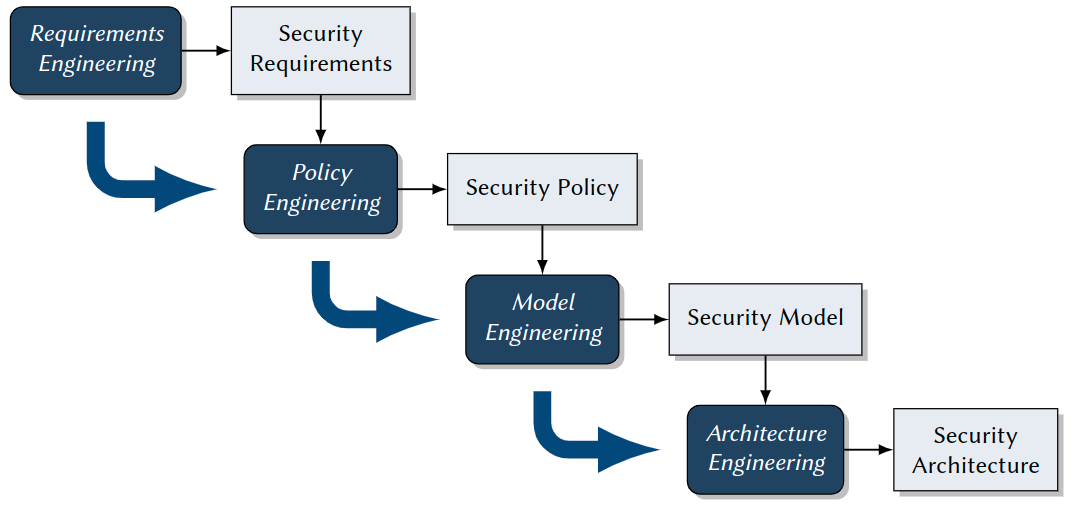
\includegraphics[width=.7\linewidth]{Assets/Systemsicherheit-engineering-process.png}
    \end{center}

    \section{Security Requirements}
    Methodology for identifying and specifying the desired security properties of an IT system.
    \begin{itemize*}
        \item Security requirements, which define what security properties a system should have.
        \item These again are the basis of a security policy: Defines how these properties are achieved
    \end{itemize*}

    Influencing Factors
    \begin{itemize*}
        \item Codes and acts (depending on applicable law)
        \begin{itemize*}
            \item EU General Data Protection Regulation (GDPR)
            \item US Sarbanes-Oxley Act (SarbOx)
        \end{itemize*}
        \item Contracts with customers
        \item Certification
        \begin{itemize*}
            \item For information security management systems (ISO 27001)
            \item Subject to German Digital Signature Act (Signaturgesetz)
        \end{itemize*}
        \item Company-specific guidelines and regulations
        \begin{itemize*}
            \item Access to critical data
            \item Permission assignment
        \end{itemize*}
        \item Company-specific infrastructure and technical requirements
        \begin{itemize*}
            \item System architecture
            \item Application systems (OSs, Database Information Systems)
        \end{itemize*}
    \end{itemize*}

    \begin{multicols}{2}
        Specialized steps in regular software requirements engineering
        \begin{enumerate*}
            \item Identify and classify vulnerabilities
            \item Identify and classify threats
            \item Match both, where relevant, to yield risks
            \item Analyze and decide which risks should be dealt with
            \item[$\rightarrow$] Fine-grained Security Requirements
        \end{enumerate*}
        \columnbreak

        \begin{center}
            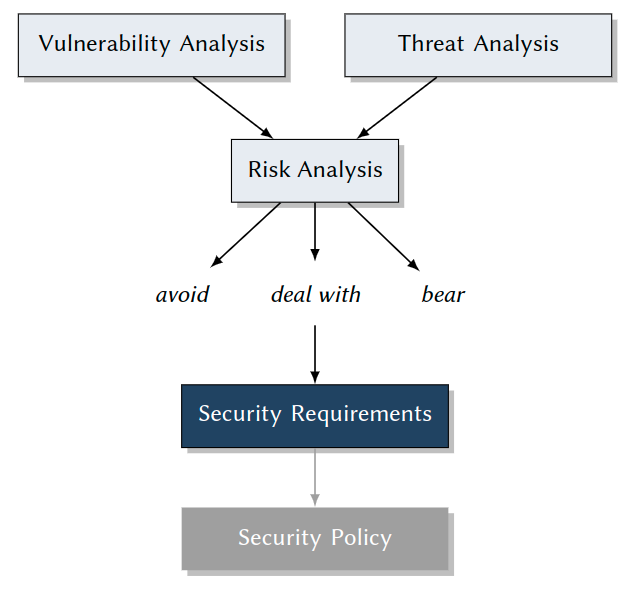
\includegraphics[width=.9\linewidth]{Assets/Systemsicherheit-risk.png}
        \end{center}
    \end{multicols}

    \subsection{Vulnerability Analysis}
    Identification of technical, organizational, human vulnerabilities of IT systems.

    \note{Vulnerability}{Feature of hardware and software constituting, an organization running, or a human operating an IT system, which is a necessary precondition for any attack in that system, with the goal to compromise one of its security properties. Set of all vulnerabilities = a system’s attack surface.}

    \subsubsection{Human Vulnerabilities}
    \begin{itemize*}
        \item Laziness
        \begin{itemize*}
            \item Passwords on Post-It
            \item Fast-clicking exercise: Windows UAC pop-up boxes
        \end{itemize*}
        \item Social Engineering
        \begin{itemize*}
            \item Pressure from your boss
            \item A favor for your friend
            \item Blackmailing: The poisoned daughter, \dots
        \end{itemize*}
        \item Lack of knowledge
        \begin{itemize*}
            \item Importing and executing malware
            \item Indirect, hidden information flow in access control systems
        \end{itemize*}
        \item Limited knowledge/skills of users
    \end{itemize*}

    \note{Social Engineering}{Influencing people into acting against their own interest or the interest of an organisation is often a simpler solution than resorting to malware or hacking.
        %Both law enforcement and the financial industry indicate that social engineering continues to enable attackers who lack the technical skills, motivation to use them or the resources to purchase or hire them. Additionally, targeted social engineering allows those technically gifted to orchestrate blended attacks bypassing both human and hardware or software lines of defence.
    }

    \subsubsection{Indirect Information Flow in Access Control Systems}

    \note{Security Requirement}{No internal information about a project, which is not approved, should ever go public}

    \note{Forbidden Information Flow}{Internal information goes into unwanted publicity}

    Problem Analysis
    \begin{itemize*}
        \item Problem complexity $\rightarrow$ effects of individual permission assignments by users to system-wide security properties
        \item Limited configuration options and granularity: archaic and inapt security mechanisms in system and application software
        \begin{itemize*}
            \item no isolation of non-trusted software
            \item no enforcement of global security policies
        \end{itemize*}
        \item[$\rightarrow$] Effectiveness of discretionary access control (DAC)
    \end{itemize*}

    \subsubsection{Organizational Vulnerabilities}
    \begin{itemize*}
        \item Access to rooms (servers)
        \item Assignment of permission on organizational level, e. g.
        \begin{itemize*}
            \item 4-eyes principle
            \item need-to-know principle
            \item definition of roles and hierarchies
        \end{itemize*}
        \item Management of cryptographic keys
    \end{itemize*}

    \subsubsection{Technical Vulnerabilities}
    The Problem: Complexity of IT Systems
    \begin{itemize*}
        \item \dots  will in foreseeable time not be
        \item Completely, consistently, unambiguously, correctly specified $\rightarrow$ contain specification errors
        \item Correctly implemented $\rightarrow$ contain programming errors
        \item Re-designed on a daily basis $\rightarrow$ contain conceptual weaknesses and vulnerabilities
        \item Weak security paradigms
    \end{itemize*}

    \subsection{Threat Analysis}
    \begin{itemize*}
        \item Identification of Attack objectives and attackers
        \item Identification of Attack methods and practices (Techniques)
        \item[$\rightarrow$] know your enemy
    \end{itemize*}

    Approach: Compilation of a threat catalog, content:
    \begin{itemize*}
        \item identified attack objectives
        \item identified potential attackers
        \item identified attack methods \& techniques
        \item damage potential of attacks
    \end{itemize*}

    \subsubsection{Attack Objectives and Attackers}
    \begin{itemize*}
        \item Economic Espionage and political power
        \begin{itemize*}
            \item Victims: high tech industry
            \item Attackers:
            \begin{itemize*}
                \item Competitors, governments, professional organizations
                \item Insiders
                \item regular, often privileged users of IT systems
            \end{itemize*}
            \item often indirect $\rightarrow$ social engineering
            \item statistical profile: age 30-40, executive function
            \item weapons: technical and organisational insider knowledge
            \item damage potential: Loss of control over critical knowledge $\rightarrow$ loss of economical or political power
        \end{itemize*}
        \item Personal Profit
        \begin{itemize*}
            \item Objective: becoming rich(er)
            \item Attackers: Competitors, Insiders
            \item damage potential: Economical damage (loss of profit)
        \end{itemize*}
        \item Wreak Havoc
        \begin{itemize*}
            \item Objective: damaging or destroying things or lives, blackmailing,\dots
            \item Attackers:
            \begin{itemize*}
                \item Terrorists: motivated by faith and philosophy, paid by organisations and governments
                \item Avengers: see insiders
                \item Psychos: all ages, all types, personality disorder
                \item[$\rightarrow$] No regular access to IT systems, no insider knowledge, but skills and tools.
            \end{itemize*}
            \item damage potential: Loss of critical infrastructures
        \end{itemize*}
        \item Meet a challenge (Hackers both good or evil)
    \end{itemize*}

    \subsubsection{Attack Methods}
    \paragraph{Scenario 1: Insider Attack}
    \begin{itemize*}
        \item Social Engineering
        \item Exploitation of conceptual vulnerabilities (DAC)
        \item Professionally tailored malware
    \end{itemize*}

    \paragraph{Scenario 2: Malware (a family heirloom \dots )}
    \begin{itemize*}
        \item Trojan horse: Executable code with hidden functionality
        \item Virus: Code for self-modification and self-duplication
        \item Logical bomb: Code that is activated by some event recognizable from the host (e. g. time, date, temperature, \dots ).
        \item Backdoor: Code that is activated through undocumented interfaces (mostly remote).
        \item Ransomware: Code for encrypting possibly all user data found on the host, used for blackmailing the victims
        \item Worm: Autonomous, self-duplicating programs
    \end{itemize*}

    \paragraph{Scenario 3: Outsider Attack}
    \begin{itemize*}
        \item Attack Method: Buffer Overflow
        \item Exploitation of implementation errors
    \end{itemize*}

    \subsubsection{Buffer Overflow Attacks}
    Privileged software can be tricked into executing attacker’s code.
    Approach: Cleverly forged parameters overwrite procedure activation frames in memory $\rightarrow$ exploitation of missing length checks on input buffers $\rightarrow$ buffer overflow

    What an Attacker Needs to Know
    \begin{itemize*}
        \item Source code of the target program, obtained by disassembling
        \item Better symbol table, as with an executable
        \item Better most precise knowledge about the compiler used (Stack)
    \end{itemize*}
    Sketch of the Attack Approach (Observations during program execution)
    \begin{itemize*}
        \item Stack grows towards the small addresses
        \item in each procedure frame: address of the next instruction to call after the current procedure returns (ReturnIP)
        \item after storing the ReturnIP, compilers reserve stack space for local variables $\rightarrow$ these occupy lower addresses
    \end{itemize*}
    Result
    \begin{itemize*}
        \item Attacker makes victim program overwrite runtime-critical parts of its stack
        \begin{itemize*}
            \item by counting up to the length of msg
            \item at the same time writing back over previously save runtime information $\rightarrow$ ReturnIP
        \end{itemize*}
        \item After finish: victim program executes code at address of ReturnIP (=address of a forged call to execute arbitrary programs)
        \item Additional parameter: file system location of a shell
    \end{itemize*}

    \note{Security Breach}{The attacker can remotely communicate, upload, download, and execute anything- with cooperation of the OS, since all of this runs with the original privileges of the victim program!}

    \paragraph{Scenario 4: High-end Malware (Root Kits)}
    \begin{itemize*}
        \item Invisible, total, sustainable takeover of a complete IT system
        \item Method: Comprehensive tool kit for fully automated attacks
        \begin{enumerate*}
            \item automatic analysis of technical vulnerabilities
            \item automated attack execution
            \item automated installation of backdoors
            \item installation and activation of stealth mechanisms
        \end{enumerate*}
        \item Target: Attacks on all levels of the software stack:
        \begin{itemize*}
            \item firmware \& bootloader
            \item operating system (e. g. file system, network interface)
            \item system applications (e. g. file and process managers)
            \item user applications (e. g. web servers, email, office)
        \end{itemize*}
        \item tailored to specific software and software versions found there
    \end{itemize*}

    \subsubsection{Root Kits}
    Step 1: Vulnerability Analysis
    \begin{itemize*}
        \item Tools look for vulnerabilities in
        \begin{itemize*}
            \item Active privileged services and demons
            \item Configuration files $\rightarrow$ Discover weak passwords, open ports
            \item Operating systems $\rightarrow$ Discover kernel and system tool versions with known implementation errors
        \end{itemize*}
        \item built-in knowledge base: automatable vulnerability database
        \item Result: System-specific collection of vulnerabilities $\rightarrow$ choice of attack method and tools to execute
    \end{itemize*}
    Step 2: Attack Execution
    \begin{itemize*}
        \item Fabrication of tailored software to exploit vulnerabilities in
        \begin{itemize*}
            \item Server processes or system tool processes (demons)
            \item OS kernel to execute code of attacker with root privileges
        \end{itemize*}
        \item This code
        \begin{itemize*}
            \item First installs smoke-bombs for obscuring attack
            \item replaces original system software by pre-fabricated modules
            \item containing backdoors or smoke bombs for future attacks
        \end{itemize*}
        \item Backdoors allow for high-privilege access in short time
        \item System modified with attacker’s servers, demons, utilities\dots
        \item Obfuscation of modifications and future access
    \end{itemize*}
    Step 3: Attack Sustainability
    \begin{itemize*}
        \item Backdoors for any further control \& command in Servers, \dots
        \item Modifications of utilities and OS to prevent
        \begin{itemize*}
            \item Killing root kit processes and connections (kill,signal)
            \item Removal of root kit files (rm,unlink)
        \end{itemize*}
        \item Results: Unnoticed access for attacker anytime, highly privileged, extremely fast, virtually unpreventable
    \end{itemize*}
    Step 4: Stealth Mechanisms (Smoke Bombs)
    \begin{itemize*}
        \item Clean logfiles (entries for root kit processes, network connections)
        \item Modify system admin utilities
        \begin{itemize*}
            \item Process management (hide running root kit processes)
            \item File system (hide root kit files)
            \item Network (hide active root kit connections)
        \end{itemize*}
        \item Substitute OS kernel modules and drivers (hide root kit processes, files, network connections), e.g. /proc/\dots , stat, fstat, pstat
        \item Processes, files and communication of root kit become invisible
    \end{itemize*}

    Risk and Damage Potential:
    \begin{itemize*}
        \item Likeliness of success: extremely highin today’s commodity OSs (High number of vulnerabilities, Speed, Fully automated)
        \item Fighting the dark arts: extremely difficult (Number and cause of vulnerabilities, weak security mechanisms, Speed, Smoke bombs)
        \item Prospects for recovering the system after successful attack $\sim 0$
    \end{itemize*}

    Countermeasure options
    \begin{itemize*}
        \item Reactive: even your OS might have become your enemy
        \item Preventive: Counter with same tools for vulnerability analysis
        \item Preventive: Write correct software
    \end{itemize*}

    \note{Security Engineering}{
        \begin{itemize*}
            \item New paradigms: policy-controlled systems $\rightarrow$ powerful software platforms
            \item New provable guarantees: formal security models $\rightarrow$ reducing specification errors and faults by design
            \item New security architectures $\rightarrow$ limiting bad effects of implementation errors and faults
        \end{itemize*}
    }

    \subsection{Risk Analysis}
    Identification and Classification of scenario-specific risks
    \begin{itemize*}
        \item Risks $\subseteq$ Vulnerabilities $\times$ Threats
        \item Correlation of vulnerabilities and threats $\rightarrow$ Risk catalogue
        \item n Vulnerabilities, m Threats $\rightarrow$ x Risks
        \item $max(n,m)<< x \leq nm$ $\rightarrow$ quite large risk catalogue
        \item Classification of risks $\rightarrow$ Complexity reduction $\rightarrow$ Risk matrix
    \end{itemize*}

    Damage Potential Assessment
    \begin{itemize*}
        \item Cloud computing $\rightarrow$ loss of confidence/reputation
        \item Industrial plant control $\rightarrow$ damage or destruction of facility
        \item Critical public infrastructure $\rightarrow$ impact on public safety
        \item Traffic management $\rightarrow$ maximum credible accident
    \end{itemize*}

    Occurrence Probability Assessment
    \begin{itemize*}
        \item Cloud computing $\rightarrow$ depending on client data sensitivity
        \item Industrial plant control $\rightarrow$ depending on plant sensitivity
        \item Critical public infrastructure $\rightarrow$ depending on terroristic threat
        \item Traffic management $\rightarrow$ depending on terroristic threat level
    \end{itemize*}

    \note{Damage potential \& Occurrence probability}{is scenario-specific}

    Depends on diverse, mostly non-technical side conditions $\rightarrow$ advisory board needed for assessment

    \paragraph{Advisory Board Output Example}
    \begin{tabular}{ p{.6cm} | l | p{.45cm} | p{4.3cm} }
        Object & Risk (Loss of\dots ) & Dmg. Pot. & Rationale                                                     \\\hline
        PD     & Integrity            & low       & Errors fast and easily detectable and correctable             \\
        PD     & Integrity            & low       & Certified software, small incentive                           \\
        PD     & Availability         & low       & Failures up to one week can be tolerated by manual procedures \\
        PD     & Availability         & med       & Certified software                                            \\
        PD     & Confidentiality      & med       & Data protection acts                                          \\
        PD     & Confidentiality      & med       & Certified software                                            \\
        TCD    & Availability         & low       & Minimal production delay, since backups are available         \\
        TCD    & Availability         & low       & Small gain by competitors or terroristic attackers            \\
        TCD    & Integrity            & med       & Medium gain by competitors or terroristic attackers           \\
        TCD    & Integrity            & high      & Production downtime                                           \\
        TCD    & Confidentiality      & high      & Huge financial gain by competitors                            \\
        TCD    & Confidentiality      & high      & Loss of market leadership                                     \\
    \end{tabular}
    PD = Personal Data; TCD = Technical Control Data

    \begin{multicols*}{2}
        \begin{center}
            Resulting Risk Matrix
            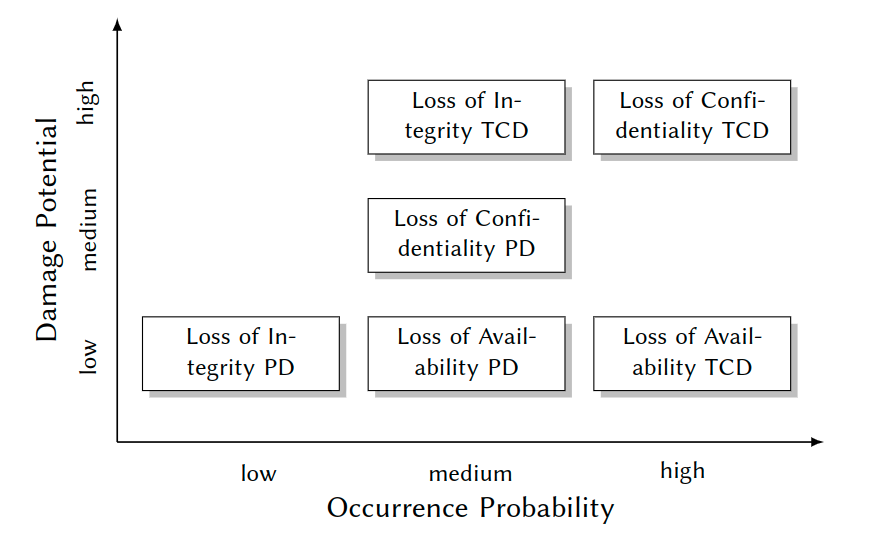
\includegraphics[width=.9\linewidth]{Assets/Systemsicherheit-risk-matrix-1.png}
        \end{center}
        \begin{center}
            Identify 3 Regions
            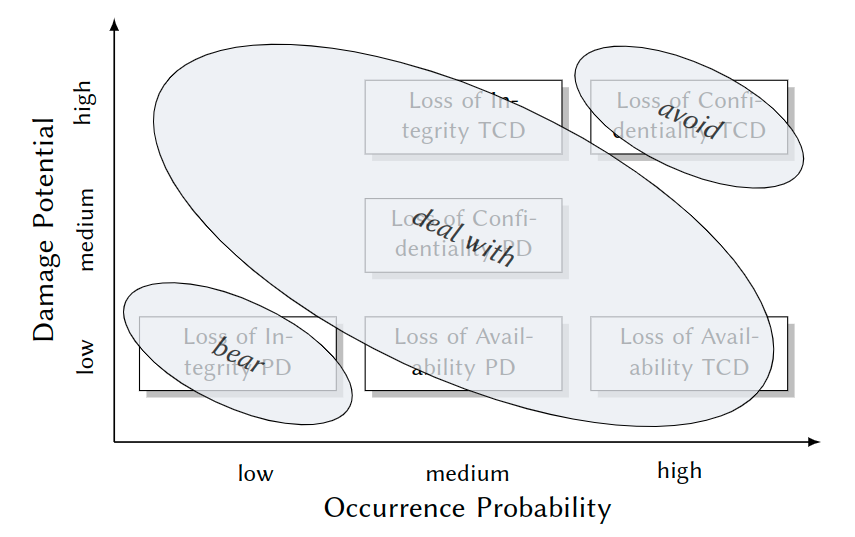
\includegraphics[width=.9\linewidth]{Assets/Systemsicherheit-Risk-Matrix-2.png}
        \end{center}
    \end{multicols*}
    \begin{itemize*}
        \item \textbf{avoid} Intolerable risk, no reasonable proportionality of costs and benefits $\rightarrow$ Don’t implement such functionality
        \item \textbf{bear} Acceptable risk $\rightarrow$ Reduce economical damage (insurance)
        \item \textbf{deal with} Risks that yield security requirements $\rightarrow$ Prevent or control by system-enforced security policies
    \end{itemize*}

    Additional Criteria:
    \begin{itemize*}
        \item Again, non-technical side conditions may apply:
        \begin{itemize*}
            \item Expenses for human resources and IT
            \item Feasibility from organizational and technological viewpoints
        \end{itemize*}
        \item[$\rightarrow$] Cost-benefit ratio: management and business experts involved
    \end{itemize*}

    \section{Security Policies and Models}
    \begin{itemize*}
        \item protect against collisions $\rightarrow$ Security Mechanisms
        \item[$\rightarrow$] Competent \& coordinated operation of mechanisms $\rightarrow$ Security Policies
        \item[$\rightarrow$] Effectiveness of mechanisms and enforcement of security policies
    \end{itemize*}

    Security Policies: a preliminary Definition
    \begin{itemize*}
        \item Malware attack $\rightarrow$ violation of confidentiality and integrity
        \item infer security requirements: Valid information flows
        \item design a security policy: Rules for controlling information flows
    \end{itemize*}

    \note{Security Policy}{a set of rules designed to meet a set of security objectives}

    \note{Security Objective}{a statement of intent to counter a given threat or to enforce a given security policy}

    Policy representations:
    \begin{itemize*}
        \item informal (natural language) text
        \item formal model
        \item functional software specification
        \item executable code
    \end{itemize*}

    How to Implement Security Policies
    \begin{itemize*}
        \item (A) Integrated in systems software ( Operating, Database)
        \item (B) Integrated in application systems
    \end{itemize*}

    \subsubsection{Implementation Alternative A}
    \begin{multicols}{2}
        The security policy is handled an OS abstractionon its own $\rightarrow$ implemented inside the kernel
        \columnbreak

        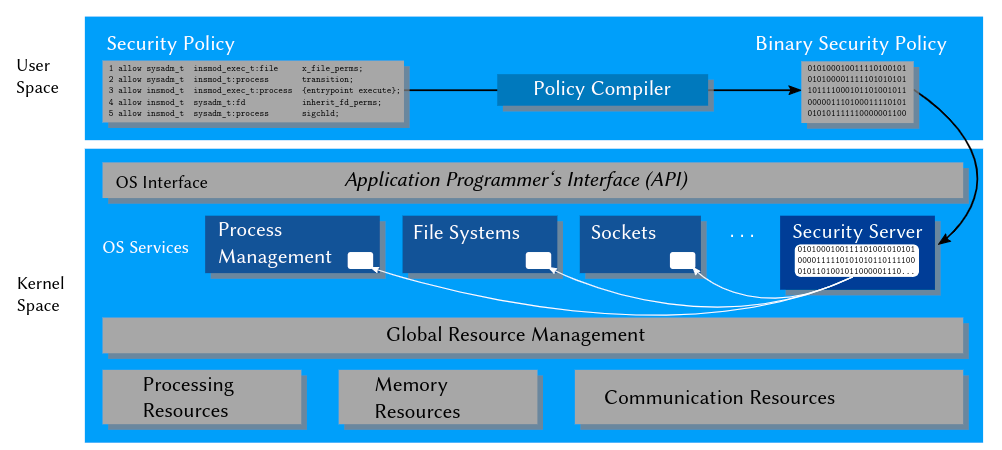
\includegraphics[width=.8\linewidth]{Assets/Systemsicherheit-pos.png}
    \end{multicols}

    Policy Enforcement in SELinux
    \begin{itemize*}
        \item \textbf{Security Server} Policy runtime environment
        \item \textbf{Interceptors} Total control of critical interactions
        \item \textbf{Policy Compiler} Translates human-readable policy modules in kernel-readable binary modules
        \item \textbf{Security Server} Manages and evaluates these modules
    \end{itemize*}

    \subsubsection{Implementation Alternative B}
    \begin{itemize*}
        \item \textbf{Application-embedded Policy} policy is only known and enforced by a user program $\rightarrow$ implemented in a user-space application
        \item \textbf{Application-level Security Architecture} policy is known and enforced by several collaborating user programs in an application systems $\rightarrow$ implemented in a local, user-space security architecture
        \item \textbf{Policy Server Embedded in Middleware} policy is communicated and enforced by several collaborating user programs in a distributed application systems $\rightarrow$ implemented in a distributed, user-space security architecture
    \end{itemize*}
    \begin{center}
        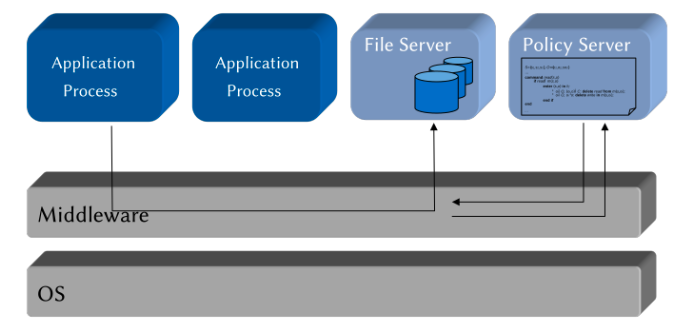
\includegraphics[width=.5\linewidth]{Assets/Systemsicherheit-application-embedded-policy.png}
    \end{center}

    \subsection{Security Models}
    Complete, unambiguous representation of security policies for
    \begin{itemize*}
        \item analyzing and explaining its behavior
        \item enabling its correct implementation
    \end{itemize*}

    How We Use Formal Models: Model-based Methodology
    \begin{itemize*}
        \item Abstraction from (too complex) reality $\rightarrow$ get rid of details
        \item Precision in describing what is significant $\rightarrow$ Model analysis and implementation
    \end{itemize*}

    \note{Security Model}{A security model is a precise, generally formal representation of a security policy.}

    Model Spectrum
    \begin{itemize*}
        \item Models for access control policies:
        \begin{itemize*}
            \item identity-based access control (IBAC)
            \item role-based access control (RBAC)
            \item attribute-based access control (ABAC)
        \end{itemize*}
        \item Models for information flow policies $\rightarrow$ multilevel security (MLS)
        \item Models for non-interference/domain isolation policies $\rightarrow$ non-interference (NI)
        \item In Practice: Most often hybrid models
    \end{itemize*}

    \subsubsection{Access Control Models}
    Formal representations of permissions to execute operations on objects

    Security policies describe access rules $\rightarrow$ security models formalize them

    \note{Identity-based access control models (IBAC)}{Rules based on the identity of individual subjects (users, processes, \dots ) or objects (files, \dots)}

    \note{Role-based access control models (RBAC)}{Rules based on roles of subjects in an organization}

    \note{Attribute-based access control models (ABAC)}{Rules based on attributes of subjects and objects}

    \note{Discretionary Access Control (DAC)}{Individual users specify access rules to objects within their area of responsibility (at their discretion).}
    Consequence: Individual users
    \begin{itemize*}
        \item granting access permissions as individually needed
        \item need to collectively enforce their organization’s security policy
        \begin{itemize*}
            \item competency problem
            \item responsibility problem
            \item malware problem
        \end{itemize*}
    \end{itemize*}

    \note{Mandatory Access Control (MAC)}{System designers and administrators specify system-wide rules, that apply for all users and cannot be sidestepped.}
    Consequence:
    \begin{itemize*}
        \item Limited individual freedom
        \item Enforced by central instance:
        \begin{itemize*}
            \item clearly identified
            \item competent (security experts)
            \item responsible (organizationally \& legally)
        \end{itemize*}
    \end{itemize*}

    \paragraph{DAC vs. MAC}
    In Real-world Scenarios: Mostly hybrid models enforced by both discretionary and mandatory components
    \begin{itemize*}
        \item \textbf{DAC} locally within a project, team members individually define permissions w. r. t. documents inside this closed scope
        \item \textbf{MAC} globally for the organization, such that e. g. only documents approved for release by organizational policy rules may be accessed from outside a project’s scope
    \end{itemize*}

    \subsubsection{Identity-based Access Control Models (IBAC)}
    To precisely specify the rights of individual, acting entities.
    \begin{center}
        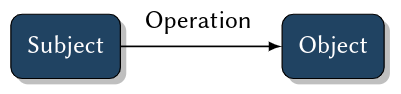
\includegraphics[width=.5\linewidth]{Assets/Systemsicherheit-ibac-basic.png}
    \end{center}
    \begin{itemize*}
        \item \textbf{Subjects}, i.e. active and identifiable entities, that execute
        \item \textbf{Operations} on
        \item passive and identifiable \textbf{Objects}, requiring
        \item \textbf{Rights} (also: permissions, privileges) which
        \begin{itemize*}
            \item control (restrict) execution of operations,
            \item are checked against identity of subjects and objects.
        \end{itemize*}
    \end{itemize*}

    Access Control Functions [Lampson, 1974]
    \begin{itemize*}
        \item basic model to define access rights: Who (subject) is allowed to do what (operation) on which object
        \item Access Control Function (ACF)
        \begin{itemize*}
            \item $f:S \times O \times OP \rightarrow \{true,false\}$ where
            \item $S$ is a set of subjects (e.g. users, processes),
            \item $O$ is a set of objects (e.g. files, sockets),
            \item $OP$ is a finite set of operations (e.g. read, write, delete)
        \end{itemize*}
        \item Interpretation: Rights to execute operations are modeled by ACF
        \begin{itemize*}
            \item any $s\in S$ represents an authenticated active entity which potentially executes operations on objects
            \item any $o\in O$ represents an authenticated passive entity on which operations are executed
            \item for any $s\in S$,$o\in O$,$op\in OP$: s is allowed to execute $op$ on $o$ iff $f(s,o,op)=true$.
            \item Model making: finding a $tuple\langle S,O,OP,f\rangle$
        \end{itemize*}
    \end{itemize*}

    \paragraph{Access Control Matrix}
    Lampson addresses how to \dots
    \begin{itemize*}
        \item store in a well-structured way,
        \item efficiently evaluate and
        \item completely analyze an ACF
    \end{itemize*}

    \note{Access Control Matrix (ACM)}{An ACM is a matrix $m:S\times O \rightarrow 2^{OP}$, such that $\forall s\in S,\forall o\in O:op\in m(s,o)\Leftrightarrow f(s,o,op)$.}

    An ACM is a rewriting of the definition of an ACF: nothing is added, nothing is left out (,,$\Leftrightarrow$'').
    \begin{itemize*}
        \item $S=\{s_1 ,\dots ,s_n\}$
        \item $O=\{o_1 ,\dots ,o_k\}$
        \item $OP=\{read,write\}$
        \item $2^{OP}=\{\varnothing,\{read\},\{write\},\{read,write\}\}^2$
        %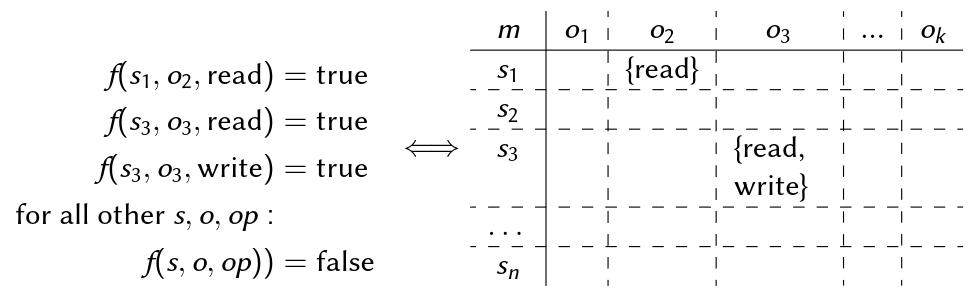
\includegraphics[width=\linewidth]{Assets/Systemsicherheit-access-control-matrix.png}
    \end{itemize*}
    \begin{itemize*}
        \item ACMs are implemented in most OS, DB, Middlewear
        \item whose security mechanisms use one of two implementations
    \end{itemize*}

    Access Control Lists (ACLs)
    \begin{itemize*}
        \item Columns of the ACM: $char*o3[N]=\{ '-', '-', 'rw', \dots \};$
        \item Found in I-Nodes of Unix, Windows, Mac OS
    \end{itemize*}

    Capability Lists
    \begin{itemize*}
        \item Rows of the ACM: $char* s1[K]=\{'-', 'r', '-', \dots \};$
        \item Found in distributed OSs, middleware, Kerberos
    \end{itemize*}

    \note{Protection State}{A fixed-time snapshot of all active entities, passive entities, and any meta-information used for making access decisions is called the protection state of an access control system.}

    ACF/ACM are to precisely specify a protection state of an AC system

    \paragraph{The Harrison-Ruzzo-Ullman Model (HRU)}

    Privilege escalation question: ,,Can it ever happen that in a given state, some specific subject obtains a specific permission?'' $\varnothing \Rightarrow \{r,w\}$
    \begin{itemize*}
        \item ACM models a single state $\langle S,O,OP,m\rangle$
        \item ACM does not tell anything about what might happen in future
        \item Behavior prediction $\rightarrow$ proliferation of rights $\rightarrow$ HRU safety
    \end{itemize*}

    We need a model which allows statements about
    \begin{itemize*}
        \item Dynamic behavior of right assignments
        \item Complexity of such an analysis
    \end{itemize*}

    Idea [Harrison et al., 1976]: A (more complex) security model combining
    \begin{itemize*}
        \item Lampson’s ACM $\rightarrow$ for modeling single protection state of an AC
        \item Deterministic automata $\rightarrow$ for modeling runtime changes of a protection state
    \end{itemize*}

    \paragraph{Deterministic Mealy Automata}
    $(Q,\sum,\Omega,\delta,\lambda,q_0)$
    \begin{itemize*}
        \item $Q$ is a finite set of states, e. g. $Q=\{q_0 ,q_1 ,q_2\}$
        \item $\sum$ is a finite set of input words, e. g. $\sum=\{a,b\}$
        \item $\Omega$ is a finite set of output words, e. g. $\Omega=\{yes,no\}$
        \item $\delta:Q\times\sum\rightarrow Q$ is the state transition function
        \item $\lambda:Q\times\sum\rightarrow\Omega$ is the output function
        \item $q_0\in Q$ is the initial state
        \item $\delta(q,\sigma)=q'$ and $\lambda(q,\sigma)=\omega$ can be expressed through the state diagram
    \end{itemize*}

    \paragraph{HRU Security Model}
    How we use Deterministic Automata
    \begin{itemize*}
        \item Snapshot of an ACM is the automaton’s state
        \item Changes of the ACM during system usage are modeled by state transitions of the automaton
        \item Effects of operations that cause such transitions are described by the state transition function
        \item Analyses of right proliferation ($\rightarrow$ privilege escalation) are enabled by state reachability analysis methods
    \end{itemize*}

    An HRU model is a deterministic automaton $\langle Q,\sum,\delta,q_0 ,R\rangle$ where
    \begin{itemize*}
        \item $Q= 2^S\times 2^O\times M$ is the state space where
        \begin{itemize*}
            \item S is a (not necessarily finite) set of subjects,
            \item O is a (not necessarily finite) set of objects,
            \item $M=\{m|m:S\times O\rightarrow 2^R\}$ is a set of possible ACMs,
        \end{itemize*}
        \item $\sum=OP\times X$ is the (finite) input alphabet where
        \begin{itemize*}
            \item $OP$ is a set of operations,
            \item $X=(S\cup O)^k$ is a set of k-dimensional vectors of arguments (subjects or objects) of these operations,
        \end{itemize*}
        \item $\sigma:Q\times\sum\rightarrow Q$ is the state transition function,
        \item $q_0\in Q$ is the initial state,
        \item R is a (finite) set of access rights.
        \item Each $q=S_q,O_q,m_q\in Q$ models a system’s protection state:
        \begin{itemize*}
            \item current subjects set $S_q\subseteq S$
            \item current objects set $O_q\subseteq O$
            \item current ACM $m_q\in M$ where $m_q:S_q\times O_q\rightarrow 2^R$
        \end{itemize*}
        \item State transitions modeled by $\delta$ based on
        \begin{itemize*}
            \item the current automaton state
            \item an input word $\langle op,(x_1,\dots ,x_k)\rangle \in\sum$ where $op$
            \item may modify $S_q$ (create a user $x_i$),
            \item may modify $O_q$ (create/delete a file $x_i$),
            \item may modify the contents of a matrix cell $m_q(x_i,x_j)$ (enter or remove rights) where $1\leq i,j\leq k$.
            \item[$\rightarrow$] We also call $\delta$ the state transition scheme (STS) of a model
        \end{itemize*}
    \end{itemize*}

    \paragraph{State Transition Scheme (STS)}
    Using the STS, $\sigma:Q\times\sum\rightarrow Q$ is defined by a set of specifications in the normalized form
    $\sigma(q,\langle op,(x_1,\dots ,x_k)\rangle )$=if $r_1\in m_q(x_{s1},x_{o1}) \wedge \dots  \wedge r_m\in m_q(x_{sm},x_{om})$ then $p_1\circ \dots \circ p_n$ where
    \begin{itemize*}
        \item $q=\{S_q,O_q,m_q\}\in Q,op\in OP$
        \item $r_1 \dots r_m\in R$
        \item $x_{s1},\dots ,x_{sm}\in S_q$ and $x_{o1},\dots ,x_{om}\in O_q$ where $s_i$ and $o_i$, $1\leq i\leq m$, are vector indices of the input arguments: $1\leq s_i,o_i\leq k$
        \item $p_1,\dots ,p_n$ are HRU primitives
        \item $\circ$ is the function composition operator: $(f\circ g)(x)=g(f(x))$
    \end{itemize*}

    Conditions: Expressions that need to evaluate ,,true'' for state q as a necessary precondition for command $op$ to be executable (= can be successfully called).

    Primitives: Short, formal macros that describe differences between $q$ and $a$ successor state $q'=\sigma(q,\langle op,(x_1 ,\dots ,x_k)\rangle )$ that result from a complete execution of op:
    \begin{itemize*}
        \item enter r into $m(x_s,x_o)$
        \item delete r from $m(x_s,x_o)$
        \item create subject $x_s$
        \item create object $x_o$
        \item destroy subject $x_s$
        \item destroy object $x_o$
        \item Each above with semantics for manipulating $S_q, O_q$ or $m_q$.
    \end{itemize*}

    Note the atomic semantics: the HRU model assumes that each command successfully called is always completely executed!

    How to Design an HRU Security Model:
    \begin{enumerate*}
        \item Model Sets: Subjects, objects, operations, rights $\rightarrow$ define the basic sets $S,O,OP,R$
        \item STS: Semantics of operations (e. g. the future API of the system to model) that modify the protection state $\rightarrow$ define $\sigma$ using the normalized form/programming syntax of the STS
        \item Initialization: Define a well-known initial state $q_0 =\langle S_0 ,O_0 ,m_0 \rangle$ of the system to model
    \end{enumerate*}

    Summary: Model Behavior
    \begin{itemize*}
        \item The model’s input is a sequence of actions from OP together with their respective arguments.
        \item The automaton changes its state according to the STS and the semantics of HRU primitives.
        \item In the initial state, each subject may (repeatedly) use a right on an object
    \end{itemize*}

    \paragraph{HRU Model Analysis}
    Analysis of Right Proliferation
    \note{HRU Safety}{(also simple-safety) A state q of an HRU model is called HRU safe with respect to a right $r\in R$ iff, beginning with q, there is no sequence of commands that enters r in an ACM cell where it did not exist in q.}

    \note{Transitive State Transition Function $\delta^*$:}{Let $\sigma\sigma\in\sum^*$ be a sequence of inputs consisting of a single input $\sigma\in\sum\cup\{\epsilon\}$ followed by a sequence $\sigma\in\sum^*$, where $\epsilon$ denotes an empty input sequence. Then, $\delta^*:Q\times\sum^*\rightarrow Q$ is defined by
        \begin{itemize*}
            \item $\delta^*(q,\sigma\sigma^*)=\delta^*(\delta(q,\sigma),\sigma^*)$
            \item $\delta^*(q,\epsilon)=q$.
        \end{itemize*}
    }

    According to Tripunitara and Li, simple-safety is defined as:
    \note{HRU Safety}{For a state $q=\{S_q,O_q,m_q\}\in Q$ and a right $r\in R$ of an HRU model $\langle Q,\sum,\delta,q_0,R\rangle$, the predicate $safe(q,r)$ holds iff
    $\forall q'= S_{q'},O_{q'},m_{q'} \in \{\delta^*(q,\sigma^*)|\sigma^*\in\sum^*\},\forall s\in S_{q'},\forall o\in O_{q'}: r\in m_{q'}(s,o)\Rightarrow s\in S_q \wedge o\in O_q \wedge r\in m_q(s,o)$.
    We say that an HRU model is safe w.r.t. r iff $safe(q_0 ,r)$.}

    showing that an HRU model is safe w.r.t. r means to
    \begin{enumerate*}
        \item Search for any possible (reachable) successor state $q'$ of $q_0$
        \item Visit all cells in $m_{q'}$ ($\forall s\in S_{q'},\forall o\in O_{q'}:\dots $)
        \item If r is found in one of these cells ($r\in m_{q'}(s,o)$), check if
        \begin{itemize*}
            \item $m_q$ is defined for this very cell ($s\in S_q\wedge o\in O_q$),
            \item $r$ was already contained in this very cell in $m_q$ ($r\in m_q\dots $).
        \end{itemize*}
        \item Recursiv. proceed with 2. for any possible successor state $q''$ of $q'$
    \end{enumerate*}

    \note{Theorem 1 [Harrison]}{Ingeneral, HRU safety is not decidable.}

    \note{Theorem 2 [Harrison]}{For mono-operational models, HRU safety is decidable.}
    \begin{itemize*}
        \item Insights into the operational principles modeled by HRU models
        \item Demonstrates a method to prove safety property for a particular, given model
        \item[$\rightarrow$] ,,Proofs teach us how to build things so nothing more needs to be proven.'' (W. E. Kühnhauser)
    \end{itemize*}

    a mono-operational HRU model $\rightarrow$ exactly one primitive for each operation in the STS

    \paragraph{Proof of Theorem - Proof Sketch}
    \begin{enumerate*}
        \item Find an upper bound for the length of all input sequences with different effects on the protection state w.r.t. safety
        If such can be found: $\exists$ a finite number of input sequences with different effects
        \item All these inputs can be tested whether they violate safety. This test terminates because:
        \begin{itemize*}
            \item each input sequence is finite
            \item there is only a finite number of relevant sequences
        \end{itemize*}
        \item[$\rightarrow$] safety is decidable
    \end{enumerate*}

    Proof: Transform $\sigma_1\dots \sigma_n$ into shorter sequences
    \begin{enumerate*}
        \item Remove all input operations that contain delete or destroy primitives (no absence, only presence of rights is checked).
        \item Prepend the sequence with an initial create subject $s_{init}$ operation.
        \item Prune the last create subject s operation and substitute each following reference to s with $s_{init}$. Repeat until all create subject operations are removed, except from the initial create subject $s_{init}$.
        \item Same as steps 2 and 3 for objects.
        \item Remove all redundant enter operations.
    \end{enumerate*}

    \begin{tabular}{l|l}
        init                       & \dots                                 \\\hline
        \dots                      & create subject $s_{init}$;            \\
        \dots                      & create object $o_{init}$              \\
        create subject $x2;$       & -                                     \\
        create object $x5;$        & -                                     \\
        enter r1 into $m(x2,x5);$  & enter r1 into $m(s_{init},o_{init})$; \\
        enter r2 into $m(x2,x5);$  & enter r2 into $m(s_{init},o_{init})$; \\
        create subject $x7;$       & -                                     \\
        delete r1 from $m(x2,x5)$; & -                                     \\
        destroy subject $x2;$      & -                                     \\
        enter r1 into $m(x7,x5);$  & -
    \end{tabular}

    Conclusions from these Theorems (Dilemma)
    \begin{itemize*}
        \item General (unrestricted) HRU models
        \begin{itemize*}
            \item have strong expressiveness $\rightarrow$ can model a broad range of AC policies
            \item are hard to analyze: algorithms and tools for safety analysis
        \end{itemize*}
        \item Mono-operational HRU models
        \begin{itemize*}
            \item have weak expressiveness $\rightarrow$ goes as far as uselessness (only create files)
            \item efficient to analyze: algorithms and tools for safety analysis
            \item[$\rightarrow$] are always guaranteed to terminate
            \item[$\rightarrow$] are straight-forward to design
        \end{itemize*}
    \end{itemize*}

    \paragraph{(A) Restricted Model Variants}

    Static HRU Models
    \begin{itemize*}
        \item Static: no create primitives allowed
        \item safe(q,r) decidable, but NP-complete problem
        \item Applications: (static) real-time systems, closed embedded systems
    \end{itemize*}

    Monotonous Mono-conditional HRU Models
    \begin{itemize*}
        \item Monotonous (MHRU): no delete or destroy primitives
        \item Mono-conditional: at most one clause in conditions part
        \item safe(q,r) efficiently decidable
        \item Applications: Archiving/logging systems (nothing is ever deleted)
    \end{itemize*}

    Finite Subject Set
    \begin{itemize*}
        \item $\forall q\in Q,\exists n\in N: |S_q|\leq n$
        \item $safe(q,r)$ decidable, but high computational complexity
    \end{itemize*}

    Fixed STS
    \begin{itemize*}
        \item All STS commands are fixed, match particular application domain (e.g. OS access control) $\rightarrow$ no model reusability
        \item For Lipton and Snyder [1977]: $safe(q,r)$ decidable in linear time
    \end{itemize*}

    Strong Type System
    \begin{itemize*}
        \item Special model to generalize HRU: Typed Access Matrix (TAM)
        \item $safe(q,r)$ decidable in polynomial time for ternary, acyclic, monotonous variants
        \item high, though not unrestricted expressiveness in practice
    \end{itemize*}

    \paragraph{(B) Heuristic Analysis Methods}
    \begin{itemize*}
        \item Restricted model variants often too weak for real-world apps
        \item General HRU models: safety property cannot be guaranteed
        \item[$\rightarrow$] get a piece from both: Heuristically guided safety estimation
    \end{itemize*}

    Idea:
    \begin{itemize*}
        \item State-space exploration by model simulation
        \item Task of heuristic: generating input sequences (educated guessing)
    \end{itemize*}

    Outline: Two-phase-algorithm to analyze $safe(q_0,r)$:
    \begin{enumerate*}
        \item Static phase: knowledge from model to make ,,good'' decisions
        \begin{itemize*}
            \item[$\rightarrow$] Runtime: polynomial in model size ($q_0 + STS$)
        \end{itemize*}
        \item Simulation phase: The automaton is implemented and, starting with $q_0$, fed with inputs $\sigma=<op,x>$
        \begin{itemize*}
            \item[$\rightarrow$] For each $\sigma$, the heuristic has to decide:
            \item which operation $op$ to use
            \item which vector of arguments $x$ to pass
            \item which $q_i$ to use from the states in $Q$ known so far
            \item Termination: As soon as $\sigma(q_i,\sigma)$ violates $safe(q_0,r)$.
        \end{itemize*}
    \end{enumerate*}

    Goal: Iteratively build up the $Q$ for a model to falsify safety by example (finding a violating but possible protection state).

    Termination: only a semi-decidable problem here. It can be guaranteed that a model is unsafe if we terminate. We cannot ever prove the opposite $\rightarrow$ safety undecidability
    \begin{itemize*}
        \item Find typical errors in security policies: Guide designers, who might know there’s something wrong but not what and why
        \item Increase understanding of unsafety origins: By building clever heuristics, we started to understand how we might design specialized HRU models that are safety-decidable yet practically (re-)usable
    \end{itemize*}

    \paragraph{The Typed-Access-Matrix Model (TAM)}
    \begin{itemize*}
        \item Adopted from HRU: subjects, objects, ACM, automaton
        \item New: leverage the principle of strong typing (like programming)
        \item[$\rightarrow$] safety decidability properties relate to type-based restrictions
        \item Foundation of a TAM model is an HRU model $\langle Q,\sum,\delta,q_0 ,R\rangle$, where $Q= 2^S\times 2^O\times M$
        \item However: $S\subseteq O$, i. e.:
        \begin{itemize*}
            \item all subjects can also act as objects (=targets of an access)
            \item useful for modeling e.g. delegation
            \item objects in $O\backslash S$: pure objects
        \end{itemize*}
        \item Each $o\in O$ has a type from a type set $T$ assigned through a mapping $type:O\rightarrow T$
        \item An HRU model is a special case of a TAM model:
        \begin{itemize*}
            \item $T=\{tSubject,tObject\}$
            \item $\forall s\in S:type(s)=tSubject; \forall o\in O\backslash S:type(o)=tObject$
        \end{itemize*}
    \end{itemize*}

    \note{TAM Security Model}{A TAM model is a deterministic automaton $\langle Q,\sum,\delta,q_0 ,T,R\rangle$ where
        \begin{itemize*}
            \item $Q= 2^S\times 2^O\times TYPE\times M$ is the state space where $S$ and $O$ are subjects set and objects set as in HRU, where $S\subseteq O$, $TYPE=\{type|type:O\rightarrow T\}$ is a set of possible type functions, $M$ is the set of possible $ACMs$ as in HRU,
            \item $\sum=OP\times X$ is the (finite) input alphabet where $OP$ is a set of operations as in HRU, $X=O^k$ is a set of $k$-dimensional vectors of arguments (objects) of these operations,
            \item $\delta:Q\times\sum\rightarrow Q$ is the state transition function,
            \item $q_0\in Q$ is the initial state,
            \item $T$ is a static (finite) set of types,
            \item $R$ is a (finite) set of access rights.
        \end{itemize*}
    }

    Convenience Notation where
    %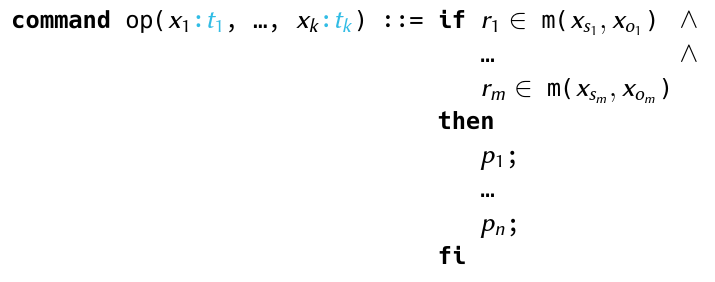
\includegraphics[width=.5\linewidth]{Assets/Systemsicherheit-tam-sts-convenience.png}
    \begin{itemize*}
        \item $q\in Q$ is implicit
        \item $op,r_1 ,\dots ,r_m,s_1 ,\dots ,s_m,o_1 ,\dots ,o_m$ as before
        \item $t_1 ,\dots ,t_k$ are argument types
        \item $p_1 ,\dots ,p_n$ are TAM-specific primitives
    \end{itemize*}

    TAM-specific
    %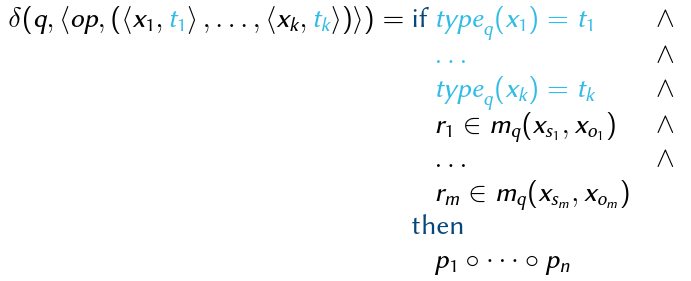
\includegraphics[width=.5\linewidth]{Assets/Systemsicherheit-tam-sts-specific.png}
    \begin{itemize*}
        \item Implicit Add-on: Type Checking where $t_i$ are the types of the arguments $x_i, 1\leq i\leq k$.
        \item Primitives:
        \begin{itemize*}
            \item enter r into m($x_s$,$x_o$)
            \item delete r from m($x_s$,$x_o$)
            \item create subject $x_s$ of type $t_s$
            \item create object $x_o$ of type $t_o$
            \item destroy subject $x_s$
            \item destroy object $x_o$
        \end{itemize*}
        \item Observation: $S$ and $O$ are dynamic (as in HRU), thus $type:O\rightarrow T$ must be dynamic too (cf. definition of $Q$ in TAM).
    \end{itemize*}

    TAM Example: The ORCON Policy
    \begin{itemize*}
        \item Creator/owner of a document should permanently retain controlover its accesses
        \item Neither direct nor indirect (by copying) right proliferation
        \item Application scenarios: Digital rights management, confidential sharing
        \item Solution with TAM: A confined subject type that can never execute any operation other than reading
    \end{itemize*}

    Model Behavior (STS): The State Transition Scheme
    \begin{itemize*}
        \item $createOrconObject(s_1:s, o_1:co)$
        \item $grantCRead(s 1 :s,s 2 :s,o 1 :co)$
        \item $useCRead(s_1:s, o_1:co, s_2:cs)$
        \item $revokeCRead(s_1:s, s_2:s, o_1:co)$
        \item $destroyOrconObject(s_1:s, o_1:co)$ (destroy conf. object)
        \item $revokeRead(s_1:s, s_2:cs, o_1:co)$ (destroy conf. subject)
        \item $finishOrconRead(s_1:s, s_2:cs)$ (destroy conf. subject)
        \item Owner retains full control over
        \item Use of her confined objects by third parties $\rightarrow$ transitive right revocation
        \item Subjects using these objects $\rightarrow$ destruction of these subjects
        \item Subjects using such objects are confined: cannot forward read information
    \end{itemize*}

    \paragraph{TAM Safety Decidability}
    \begin{itemize*}
        \item General TAM models $\rightarrow$ safety not decidable
        \item \textbf{MTAM} monotonous TAM models; STS without delete or destroy primitives $\rightarrow$ safety decidable if mono-conditional only
        \item \textbf{AMTAM} acyclic MTAM models $\rightarrow$ safety decidable but not efficiently (NP-hard problem)
        \item \textbf{TAMTAM} ternary AMTAM models; each STS command requires max. 3 arguments $\rightarrow$ provably same computational power and thus expressive power as AMTAM; safety decidable in polynomial time
    \end{itemize*}

    \paragraph{Acyclic TAM Models}

    \note{Parent- and Child-Types}{For any operation $op$ with arguments $\langle x_1,t_1\rangle ,\dots ,\langle x_k,t_k\rangle$ in an STS of a TAM model, it holds that $t_i, 1\leq i\leq k$
        \begin{itemize*}
            \item is a child type in op if one of its primitives creates a subject or object $x_i$ of type $t_i$,
            \item is a parent type in op if none of its primitives creates a subject or object $x_i$ of type $t_i$.
        \end{itemize*}
    }

    \note{Type Creation Graph}{The type creation graph $TCG=\langle T,E=T\times T\rangle$ for the STS of a TAM model is a directed graph with vertex set $T$ and an $edge\langle u,v\rangle \in E$ iff $\exists op\in OP:u$ is a parent type in $op\wedge v$ is a child type in op.}

    \begin{multicols}{2}
        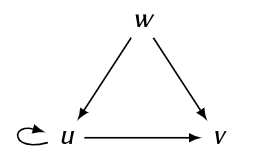
\includegraphics[width=.7\linewidth]{Assets/Systemsicherheit-acyclic-tam-example.png}
        \columnbreak

        Note: In bar $u$ is both a parent type (because of $s_1$) and a child type (because of $s_2$) $\rightarrow$ hence the loop edge.
    \end{multicols}

    Safety Decidability: We call a TAM model acyclic, iff its TCG is acyclic.

    \note{Theorem 5}{Safety of a ternary, acyclic, monotonous TAM model (TAMTAM) is decidable in polynomial time in the size of $m_0$.}

    Crucial property acyclic, intuitively:
    \begin{itemize*}
        \item Evolution of the system (protection state transitions) checks both rights in the ACM as well as argument types
        \item TCG is acyclic $\Rightarrow\exists$ a finite sequence of possible state transitions after which no input tuple with argument types, that were not already considered before, can be found
        \item One may prove that an algorithm, which tries to expandall possible different follow-up states from $q_0$, may terminate after this finite sequence
    \end{itemize*}

    Expressive Power of TAMTAM
    \begin{itemize*}
        \item MTAM: obviously same expressive power as monotonic HRU
        \begin{itemize*}
            \item no transfer of rights: ,,take r \dots  in turn grant r to \dots ''
            \item no countdown rights: ,,r can only be used n times''
        \end{itemize*}
        \item ORCON: allow to ignore non-monotonic command $s$ from STS since they only remove rights and are reversible
        \item AMTAM: most MTAM STS may be re-written as acyclic
        \item TAMTAM: expressive power equivalent to AMTAM
    \end{itemize*}

    \begin{multicols}{2}
        IBAC Model Comparison: family of IBAC models to describe different ranges of security policies they are able to express \columnbreak

        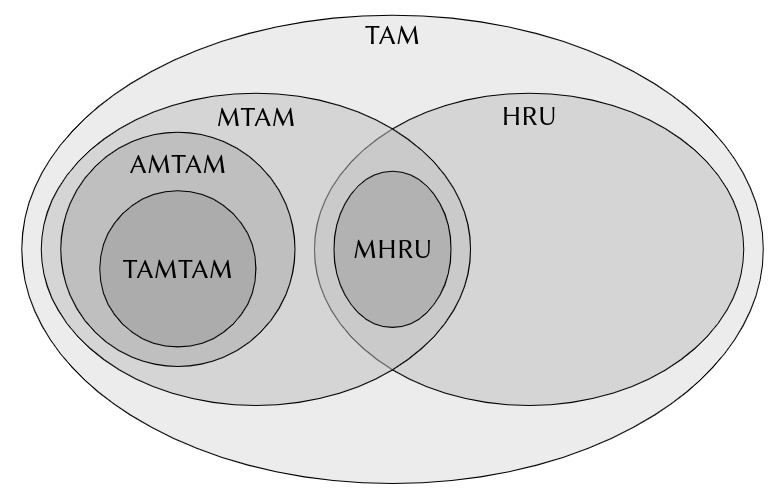
\includegraphics[width=.5\linewidth]{Assets/Systemsicherheit-ibac-model-comparison.png}
    \end{multicols}

    \subsubsection{Roles-based Access Control Models (RBAC)}
    Solving Scalability and Abstraction results in smaller modeling effort results in smaller chance of human errors made in the process
    \begin{itemize*}
        \item Improved scalability and manageability
        \item application-oriented semantic: $roles\approx functions$ in organizations
        \item Models include smart abstraction: roles
        \item AC rules are specified based on roles instead of identities
        \item Users, roles, and rights for executing operations
        \item Access rules are based on roles of users $\rightarrow$ on assignments
        \item improved Scalability
        \item improved Application-oriented model abstractions
        \item Standardization (RBAC96) $\rightarrow$ tool-support
        \item Limited dynamic analyses w.r.t. automaton-based models
    \end{itemize*}

    \note{Basic RBAC model}{An $RBAC_0$ model is a tuple $\langle U,R,P,S,UA,PA,user,roles\rangle$ where
        \begin{itemize*}
            \item U is a set of user identifiers,
            \item R is a set of role identifiers,
            \item P is a set of permission identifiers,
            \item S is a set of session identifiers,
            \item $UA\subseteq U\times R$ is a many-to-many user-role-relation,
            \item $PA\subseteq P\times R$ is a many-to-many permission-role-relation,
            \item $user:S\rightarrow U$ is a total function mapping sessions to users,
            \item $roles:S\rightarrow 2^R$ is a total function mapping sessions to sets of roles such that $\forall s\in S:r\in roles(s)\Rightarrow \langle user(s),r\rangle \in UA$.
        \end{itemize*}
    }

    Interpretation
    \begin{itemize*}
        \item Users U model people: actual humans that operate the AC system
        \item Roles R model functions, originate from workflows/responsibility
        \item Permissions P model rights for any particular access
        \item user-role-relation $UA\subseteq U\times R$ defines which roles are available to users at any given time $\rightarrow$ assumed during runtime before usable
        \item permission-role-relation $PA\subseteq P\times R$
        \item $UA$ and $PA$ describe static policy rules
        \item Sessions $S$ describe dynamic assignments of roles $\rightarrow$ a session $s\in S$ models when a user is logged in
        \begin{itemize*}
            \item $S\rightarrow U$ associates a session with its (,,owning'') user
            \item $S\rightarrow 2^R$ associates a session with the set of roles currently assumed by that user (active roles)
        \end{itemize*}
    \end{itemize*}
    \begin{center}
        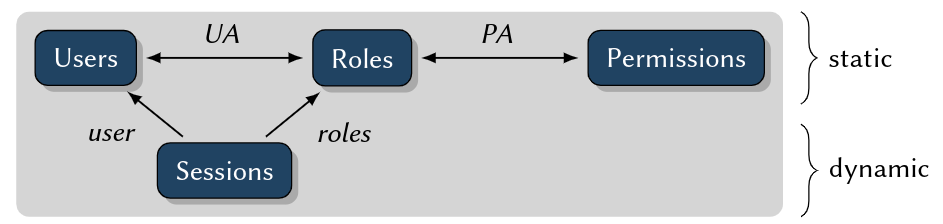
\includegraphics[width=.5\linewidth]{Assets/Systemsicherheit-rbac-0.png}
    \end{center}

    \paragraph{RBAC Access Control Function}
    \begin{itemize*}
        \item access rules have to be defined for operations on objects
        \item implicitly defined through $P\rightarrow$ made explicit: $P\subseteq O\times OP$ is a set of permission tuples $\langle o,op\rangle$ where
        \begin{itemize*}
            \item $o\in O$ is an object from a set of object identifiers,
            \item $op\in OP$ is an operation from a set of operation identifiers.
        \end{itemize*}
        \item We may now define the $ACF$ for $RBAC_0$
    \end{itemize*}

    \note{$RBAC_0$ ACF}{
        $f_{RBAC_0}:U \times O\times OP\rightarrow\{true,false\}$ where
        $\begin{cases} true, \quad \exists r\in R,s\in S:u=user(s)\wedge r\in roles(s)\wedge \langle \langle o,op\rangle ,r\rangle \in PA \\ false, \quad\text{ otherwise } \end{cases}$
    }

    \paragraph{RBAC96 Model Family}
    In practice, organizations have more requirements that need to be expressed in their security policy
    \begin{itemize*}
        \item $RBAC_1 = RBAC_0 + hierarchies$
        \item $RBAC_2 = RBAC_0 + constraints$
        \item $RBAC_3 = RBAC_0 + RBAC_1 + RBAC_2$
    \end{itemize*}

    \paragraph{RBAC 1: Role Hierarchies}
    Roles often overlap
    \begin{enumerate*}
        \item disjoint permissions for roles $\rightarrow$ any user X must always have Y assigned and activated for any of her workflows $\rightarrow$ role assignment redundancy
        \item overlapping permissions: $\forall p\in P:\langle p,proDev\rangle \in PA\Rightarrow \langle p,proManager\rangle \in PA\rightarrow$ any permission must be assigned to two different roles $\rightarrow$ role definition redundancy
        \item Two types of redundancy $\rightarrow$ undermines scalability goal of RBAC
    \end{enumerate*}

    Solution: Role hierarchy $\rightarrow$ Eliminates role definition redundancy through permissions inheritance

    Modeling Role Hierarchies: Lattice here: $\langle R,\leq\rangle$
    \begin{itemize*}
        \item Hierarchy expressed through dominance relation: $r_1\leq r_2 \Leftrightarrow r_2$ inherits any permissions from $r_1$
        \item \textbf{Reflexivity} any role consists of its own permissions
        \item \textbf{Antisymmetry} no two different roles may mutually inherit their respective permissions
        \item \textbf{Transitivity} permissions may be inherited indirectly
    \end{itemize*}

    \note{$RBAC_1$ Security Model}{An $RBAC_1$ model is a tuple $\langle U,R,P,S,UA,PA,user,roles,RH\rangle$ where
        \begin{itemize*}
            \item $U,R,P,S,UA,PA$ and $user$ are defined as for $RBAC_0$,
            \item $RH\subseteq R\times R$ is a partial order that represents a role hierarchy where $\langle r,r'\rangle \in RH\Leftrightarrow r\leq r'$ such that $\langle R,\leq\rangle$ is a lattice,
            \item roles is defined as for $RBAC_0$, while additionally holds: $\forall r,r'\in R,\exists s\in S:r\leq r'\wedge r'\in roles(s)\Rightarrow r\in roles(s)$.
        \end{itemize*}
    }

    \paragraph{RBAC 2: Constraints}
    roles in org. often more restricted
    \begin{itemize*}
        \item Certain roles may not be active at the same time (session) for any user
        \item Certain roles may not be together assigned to any user
        \item[$\rightarrow$] separation of duty (SoD)
        \item While SoD constraints are a more fine-grained type of security requirements to avoid mission-critical risks, there are other types represented by RBAC constraints
    \end{itemize*}
    Constraint Types
    \begin{itemize*}
        \item \textbf{Separation of duty} mutually exclusive roles
        \item \textbf{Quantitative constraints} maximum number of roles per user
        \item \textbf{Temporal constraints} time/date/week/\dots  of role activation
        \item \textbf{Factual constraints} assigning or activating roles for specific permissions causally depends on any roles for a certain
    \end{itemize*}
    Modeling Constraints Idea
    \begin{itemize*}
        \item $RBAC_2: \langle U,R,P,S,UA,PA,user,roles,RE\rangle$
        \item $RBAC_3: \langle U,R,P,S,UA,PA,user,roles,RH,RE\rangle$
        \item where $RE$ is a set of logical expressions over the other model components (such as $UA,PA,user,roles$)
    \end{itemize*}

    \subsubsection{Attribute-based Access Control Models (ABAC)}
    \begin{itemize*}
        \item Scalability and manageability
        \item Application-oriented model abstractions
        \item Model semantics meet functional requirements of open systems:
        \begin{itemize*}
            \item user IDs, INode IDs, \dots only available locally
            \item roles limited to specific organizational structure
        \end{itemize*}
        \item[$\rightarrow$] application-specific context of access: attributes of subjects and objects (e. g. age, location, trust level, \dots )
    \end{itemize*}

    Idea: Generalizing the principle of indirection already known from RBAC
    \begin{itemize*}
        \item IBAC: no indirection between subjects and objects
        \item RBAC: indirection via roles assigned to subjects
        \item ABAC: indirection via arbitrary attributes assigned to sub-/objects
        \item Attributes model application-specific properties of the system entities involved in any access
        \begin{itemize*}
            \item Age, location, trustworthiness of a application/user/\dots
            \item Size, creation time, access classification of resource/\dots
            \item Risk quantification involved with these subjects and objects
        \end{itemize*}
    \end{itemize*}

    \paragraph{ABAC Access Control Function}
    \begin{itemize*}
        \item $f_{IBAC}:S\times O\times OP\rightarrow\{true,false\}$
        \item $f_{RBAC}:U\times O\times OP\rightarrow\{true,false\}$
        \item $f_{ABAC}:S\times O\times OP\rightarrow\{true,false\}$
        \item[$\rightarrow$] Evaluates attribute values for $\langle s,o,op\rangle$
    \end{itemize*}

    \paragraph{ABAC Security Model}
    \begin{itemize*}
        \item Note: There is no such thing (yet) like a standard ABAC model
        \item Instead: Many highly specialized, application-specific models.
        \item Here: minimal common formalism, based on Servos and Osborn
    \end{itemize*}

    \note{ABAC Security Model}{An ABAC security model is a tuple $\langle S,O,AS,AO,attS,attO,OP,AAR\rangle$ where
        \begin{itemize*}
            \item $S$ is a set of subject identifiers and $O$ is a set of object identifiers,
            \item $A_S=V_S^1 \times\dots \times V_S^n$ is a set of subject attributes, where each attribute is an n-tuple of values from arbitrary domains $V_S^i$, $1\leq i \leq n$,
            \item $A_O=V_O^1\times\dots \times V_O^m$ is a corresponding set of object attributes, based on values from arbitrary domains $V_O^j$, $1\leq j \leq m$,
            \item $att_S:S\rightarrow A_S$ is the subject attribute assignment function,
            \item $att_O:O\rightarrow A_O$ is the object attribute assignment function,
            \item $OP$ is a set of operation identifiers,
            \item $AAR\subseteq \Phi\times OP$ is the authorization relation.
        \end{itemize*}
    }

    Interpretation
    \begin{itemize*}
        \item Active and passive entities are modeled by $S$ and $O$, respectively
        \item Attributes in $AS,AO$ are index-referenced tuples of values, which are specific to some property of subjects $V_S^i$ (e.g. age) or of objects $V_O^j$ (e. g. PEGI rating)
        \item Attributes are assigned to subjects and objects via $att_S,att_O$
        \item Access control rules w.r.t. the execution of operations in $OP$ are modeled by the $AAR$ relation $\rightarrow$ determines ACF!
        \item $AAR$ is based on a set of first-order logic predicates $\Phi$: $\Phi=\{\phi_1 (x_{s1},x_{o1}),\phi_2 (x_{s2},x_{o2}),\dots \}$. Each $\phi_i\in\Phi$ is a binary predicate, where $x_{si}$ is a subject variable and $x_{oi}$ is an object variable.
    \end{itemize*}

    \note{ABAC Access Control Function (ACF)}{
        \begin{itemize*}
            \item $f_{ABAC}:S\times O\times OP\rightarrow\{true,false\}$ where
            \item $f_{ABAC}(s,o,op)= \begin{cases} true, \quad\exists \langle \phi,op\rangle \in AAR:\phi(s,o)=true\\ false, \quad\text{ otherwise } \end{cases}$.
            \item We call $\phi$ an authorization predicate for $op$.
        \end{itemize*}
    }

    \subsubsection{Information Flow Models (IF)}
    Abstraction level of AC Models: rules about subjects accessing objects.

    Goal: Problem-oriented definition of policy rules for scenarios based on information flows(rather than access rights)
    \begin{itemize*}
        \item Information flows and read/write operations are isomorphic
        \begin{itemize*}
            \item s has read permission o $\Leftrightarrow$ information flow from o to s
            \item s has write permission o $\Leftrightarrow$ information flow from s to o
        \end{itemize*}
        \item[$\rightarrow$] Implementation by standard AC mechanisms!
    \end{itemize*}

    Analysis of Information Flow Models
    \begin{itemize*}
        \item IF Transitivity $\rightarrow$ goal: covert information flows
        \item IF Antisymmetry $\rightarrow$ goal: redundancy
    \end{itemize*}

    \note{Denning Security Model}{A Denning information flow model is a tuple $\langle S,O,L,cl,\bigoplus\rangle$ where
        \begin{itemize*}
            \item S is a set of subjects,
            \item O is a set of objects,
            \item $L=\langle C,\leq\rangle$ is a lattice where
            \begin{itemize*}
                \item C is a set of classes,
                \item $\leq$ is a dominance relation where c $\leq d \Leftrightarrow$ information may flow from c to d,
            \end{itemize*}
            \item $cl:S\cup O\rightarrow C$ is a classification function, and
            \item $\bigoplus:C\times C\rightarrow C$ is a reclassification function.
        \end{itemize*}
    }

    Interpretation
    \begin{itemize*}
        \item Subject set S models active entities, which information flows originate from
        \item Object set O models passive entities, which may receive information flows
        \item Classes set C used to label entities with identical information flow properties
        \item Classification function $cl$ assigns a class to each entity
        \item Reclassification function $\bigoplus$ determines which class an entity is assigned after receiving certain a information flow
    \end{itemize*}
    This enables
    \begin{itemize*}
        \item precisely define all information flows valid for a given policy
        \item define analysis goals for an IF model w.r.t.
        \begin{itemize*}
            \item \textbf{Correctness} $\exists$ covert information flows?
            \item \textbf{Redundancy} $\exists$ sets of subjects and objects with equivalent information contents?
        \end{itemize*}
        \item implement a model through an automatically generated, isomorphic ACM
    \end{itemize*}

    \subsubsection{Multilevel Security (MLS)}
    \begin{itemize*}
        \item Introducing a hierarchy of information flow classes: levels of trust
        \item Subjects and objects are classified:
        \begin{itemize*}
            \item Subjects w.r.t. their trust worthiness
            \item Objects w.r.t. their criticality
        \end{itemize*}
        \item Within this hierarchy, information may flow only in one direction $\rightarrow$ ,,secure'' according to these levels!
        \item $\rightarrow \exists$ MLS models for different security goals!
    \end{itemize*}

    Modeling Confidentiality Levels
    \begin{itemize*}
        \item Class set: levels of confidentiality e.g. $C=\{public,conf,secret\}$
        \item Dominance relation: hierarchy between confidentiality levels e.g. $\{public \leq confidential,confidential \leq secret\}$
        \item Classification of subjects and objects: $cl:S\cup O\rightarrow C$ e.g. $cl(BulletinBoard)=public,cl(Timetable)=confidential$
        \item In contrast due Denning $\leq$ in MLS models is a total order
    \end{itemize*}

    \paragraph{The Bell-LaPadula Model}
    MLS-Model for Preserving Information Confidentiality.
    Incorporates impacts on model design \dots
    \begin{itemize*}
        \item from the application domain: hierarchy of trust
        \item from the Denning model: information flow and lattices
        \item from the MLS models: information flow hierarchy
        \item from the HRU model:
        \begin{itemize*}
            \item Modeling dynamic behavior: state machine and STS
            \item Model implementation: ACM
        \end{itemize*}
        \item[$\rightarrow$] application-oriented model engineering by composition of known abstractions
    \end{itemize*}

    \note{BLP Security Model}{A BLP model is a deterministic automaton $\langle S,O,L,Q,\sum,\sigma,q_0,R\rangle$ where
        \begin{itemize*}
            \item S and O are (static) subject and object sets,
            \item $L=\langle C,\leq\rangle$ is a (static) lattice consisting of
            \begin{itemize*}
                \item the classes set C,
                \item the dominance relation $\leq$,
            \end{itemize*}
            \item $Q=M\times CL$ is the state space where
            \begin{itemize*}
                \item $M=\{m|m:S\times O\rightarrow 2^R\}$ is the set of possible ACMs,
                \item $CL=\{cl|cl:S\cup O\rightarrow C\}$ is a set of functions that classify entities in $S\cup O$,
            \end{itemize*}
            \item $\sum$ is the input alphabet,
            \item $\sigma:Q\times \sum\rightarrow Q$ is the state transition function,
            \item $q_0\in Q$ is the initial state,
            \item $R=\{read,write\}$ is the set of access rights.
        \end{itemize*}
    }

    Interpretation
    \begin{itemize*}
        \item $S,O,M,\sum,\sigma,q_0,R$: same as HRU
        \item L: models confidentiality hierarchy
        \item cl: models classification meta-information about sub-/objects
        \item $Q=M\times CL$ models dynamic protection states; includes
        \begin{itemize*}
            \item rights in the ACM,
            \item classification of subjects/objects,
            \item not: S and O (different to HRU)
        \end{itemize*}
        \item Commands in the STS may therefore
        \begin{itemize*}
            \item change rights in the ACM,
            \item reclassify subjects and objects.
        \end{itemize*}
    \end{itemize*}
    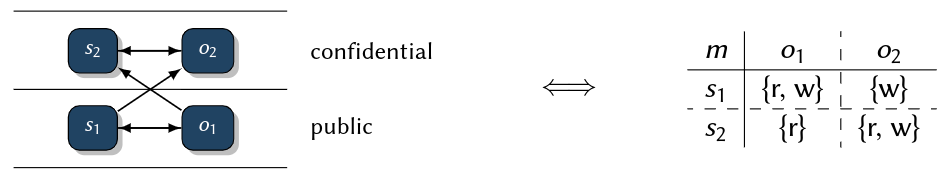
\includegraphics[width=\linewidth]{Assets/Systemsicherheit-lattice-vs-acm.png}

    \begin{itemize*}
        \item L is an application-oriented abstraction
        \begin{itemize*}
            \item Supports convenient for model specification
            \item Supports easy model correctness analysis
            \item[$\rightarrow$] easy to specify and to analyze
        \end{itemize*}
        \item m can be directly implemented by standard OS/DBIS access control mechanisms (ACLs, Capabilities) $\rightarrow$ easy to implement
        \item m is determined (= restricted) by L and cl, not vice-versa
        \item L and cl control m
    \end{itemize*}

    \subsubsection{BLP Security}
    \note{Read-Security Rule}{A BLP model state $\langle m,cl\rangle$ is called read-secure iff $\forall s\in S,o\in O:read\in m(s,o)\Rightarrow cl(o) \leq cl(s)$.}

    \note{Write-Security Rule}{A BLP model state $\langle m,cl\rangle$ is called write-secure iff $\forall s\in S,o\in O:write\in m(s,o)\Rightarrow cl(s)\leq cl(o)$.}

    \note{State Security}{A BLP model state is called secure iff it is both read- and write-secure.}

    \note{Model Security}{A BLP model with initial state $q_0$ is called secure iff
        \begin{enumerate*}
            \item $q_0$ is secure and
            \item each state reachable from $q_0$ by a finite input sequence is secure.
        \end{enumerate*}
    }

    \note{BLP Basic Security Theorem}{A BLP model $\langle S,O,L,Q,\sum,\sigma,q_0,R\rangle$ is secure iff both of the following holds:
        \begin{enumerate*}
            \item $q_0$ is secure
            \item $\sigma$ is build such that for each state q reachable from $q_0$ by a finite input sequence, where $q=\langle m,cl\rangle$ and $q'=\sigma(q,\delta)=m',cl',\forall s\in S, o\in O,\delta\in\sum$ the following holds:
        \end{enumerate*}
        \begin{itemize*}
            \item Read-security conformity:
            \begin{itemize*}
                \item read $\not\in m(s,o)\wedge read\in m'(s,o)\Rightarrow cl'(o)\leq cl'(s)$
                \item read $\in m(s,o) \wedge\lnot (cl'(o)\leq cl'(s)) \Rightarrow read \not\in m'(s,o)$
            \end{itemize*}
            \item Write-security conformity:
            \begin{itemize*}
                \item write $\not\in m(s,o)\wedge write \in m'(s,o)\Rightarrow cl'(s)\leq cl'(o)$
                \item write $\in m(s,o)\wedge\lnot(cl'(s)\leq cl'(o)) \Rightarrow write \not\in m'(s,o)$
            \end{itemize*}
        \end{itemize*}
    }

    Idea: Encode an additional, more fine-grained type of access restriction in the ACM $\rightarrow$ compartments
    \begin{itemize*}
        \item Comp: set of compartments
        \item $co:S\cup O\rightarrow 2^{Comp}$: assigns a set of compartments to an entity as an (additional) attribute
        \item Refined state security rules:
        \begin{itemize*}
            \item $\langle m,cl,co\rangle$ is read-secure $\Leftrightarrow\forall s\in S,o\in O:read \in m(s,o)\Rightarrow cl(o)\leq cl(s)\wedge co(o) \subseteq co(s)$
            \item $\langle m,cl,co\rangle$ is write-secure $\Leftrightarrow\forall s\in S,o\in O:write\in m(s,o)\Rightarrow cl(s)\leq cl(o)\wedge co(o) \subseteq co(s)$
        \end{itemize*}
        \item BLP with compartments: $\langle S,O,L,Comp,Q_{co},\sigma,\delta,q_0\rangle$ where $Q_{co}=M\times CL\times CO$ and $CO=\{co|co:S\cup O\rightarrow 2^{Comp}\}$
    \end{itemize*}

    \paragraph{BLP Model Summary}
    \begin{itemize*}
        \item Application-oriented modeling $\rightarrow$ hierarchical information flow
        \item Scalability $\rightarrow$ attributes: trust levels
        \item Modeling dynamic behavior $\rightarrow$ automaton with STS
        \item Correctness guarantees (analysis of)
        \begin{itemize*}
            \item consistency: BLP security, BST
            \item completeness of IF: IFG path finding
            \item presence of unintended IF: IFG path finding
            \item unwanted redundancy: IF cycles
            \item safety properties: decidable
        \end{itemize*}
        \item Implementation
        \begin{itemize*}
            \item ACM is a standard AC mechanism in contemporary implementation platforms (cf. prev. slide)
            \item Contemporary standard OSs need this: do not support mechanisms for entity classification, arbitrary STSs
            \item new platforms: SELinux, TrustedBSD, PostgreSQL, \dots
        \end{itemize*}
        \item Is an example of a hybrid model: IF + AC + ABAC
    \end{itemize*}

    \subsubsection{The Biba Model}
    \begin{multicols}{2}
        BLP upside down
        \begin{itemize*}
            \item BLP $\rightarrow$ preserves confidentiality
            \item Biba $\rightarrow$ preserves integrity
        \end{itemize*}
        \columnbreak

        \begin{center}
            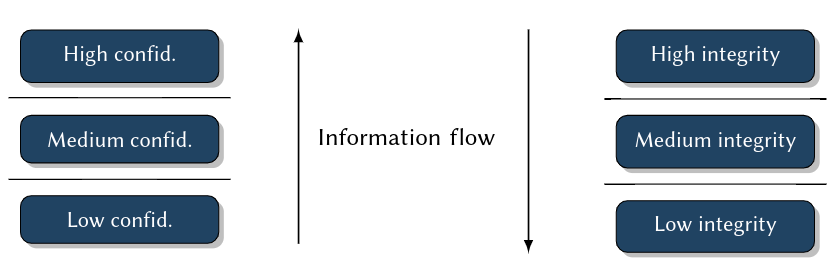
\includegraphics[width=\linewidth]{Assets/Systemsicherheit-blp-vs-biba.png}
        \end{center}
    \end{multicols}

    OS Example: file/process/\dots created is classified $\rightarrow$ cannot violate integrity of objects

    \subsubsection{Non-interference Models (NI)}
    Problems: Covert Channels \& Damage Range (Attack Perimeter)

    \note{Covert Channel}{Channels not intended for information transfer at all, such as the service program’s effect on the system load.}

    \begin{itemize*}
        \item AC policies (ACM, HRU, TAM, RBAC, ABAC): colluding malware agents, escalation of common privileges
        \begin{itemize*}
            \item Process 1: only read permissions on user files
            \item Process 2: only permission to create an internet socket
            \item both: communication via covert channel
        \end{itemize*}
        \item MLS policies (Denning, BLP, Biba): indirect information flow exploitation (can never prohibitany possible transitive IF \dots )
        \begin{itemize*}
            \item Test for existence of a file
            \item Volume control on smartphones
        \end{itemize*}
    \end{itemize*}

    Idea of NI models
    \begin{itemize*}
        \item higher level of abstraction
        \item which domains should be isolated based on their mutual impact
        \item[$\rightarrow$] Easier policy modeling
        \item[$\rightarrow$] More difficult implementation $\rightarrow$ higher degree of abstraction
        \item Needed: isolation of services, restricted cross-domain interactions
        \item[$\rightarrow$] Guarantee of total/limited non-interference between domains
    \end{itemize*}

    \paragraph{NI Security Policies}
    Security domains \& Cross-domain actions

    \note{Non-Interference}{Two domains do not interfere with each other iff no action in one domain can be observed by the other.}

    \note{NI Security Model}{An NI model is a det. automaton $\langle Q,\sigma,\delta,\lambda,q_0,D,A,dom,\approx_{NI},Out\rangle$ where
        \begin{itemize*}
            \item Q is the set of (abstract) states,
            \item $\sigma=A$ is the input alphabet where A is the set of (abstract) actions,
            \item $\delta:Q\times\sigma\rightarrow Q$ is the state transition function,
            \item $\lambda:Q\times\sigma\rightarrow Out$ is the output function,
            \item $q_0\in Q$ is the initial state,
            \item $D$ is a set of domains,
            \item $dom:A\rightarrow 2^D$ is adomain function that completely defines the set of domains affected by an action,
            \item $\approx_{NI}\subseteq D\times D$ is a non-interference relation,
            \item $Out$ is a set of (abstract) outputs.
        \end{itemize*}
        NI Security Model is also called Goguen/Meseguer-Model.
    }

    BLP written as an NI Model
    \begin{itemize*}
        \item BLP Rules:
        \begin{itemize*}
            \item write in class public may affect public and confidential
            \item write in class confidential may only affect confidential
        \end{itemize*}
        \item NI Model:
        \begin{itemize*}
            \item $D=\{d_{pub},d_{conf}\}$
            \item write in $d_{conf}$ does not affect $d_{pub}$, so $d_{conf} \approx_{NI} d_{pub}$
            \item $A=\{writeInPub, writeInConf\}$
            \item $dom(writeInPub)=\{d_{pub},d_{conf}\}$
            \item $dom(writeInConf)=\{d_{conf}\}$
        \end{itemize*}
    \end{itemize*}

    \paragraph{NI Model Analysis}

    \note{Purge Function}{Let $aa^*\in A^*$ be a sequence of actions consisting of a single action $a\in A\cup\{\epsilon\}$ followed by a sequence $a^*\in A^*$, where $\epsilon$ denotes an empty sequence. Let $D'\in 2^D$ be any set of domains. Then, purge: $A^*\times 2^D \rightarrow A^*$ computes a subsequence of $aa^*$ by removing such actions without an observable effect on any element of $D':$
        \begin{itemize*}
            \item $purge(aa^*,D')=\begin{cases} a\circ purge(a^*,D'), \exists d_a\in dom(a),d'\in D':d_a\approx_I d' \\ purge(a^*,D'), \quad\text{ otherwise }\end{cases}$
            \item $purge(\epsilon,D')=\epsilon$
        \end{itemize*}
        where $\approx_I$ is the complement of $\approx_{NI}:d_1 \approx_I d_2\Leftrightarrow \lnot(d_1 \approx_{NI} d_2)$.
    }

    \note{NI Security}{For a state $q\in Q$ of an NI model $\langle Q,\sigma,\delta,\lambda,q_0,D,A,dom,\approx_{NI},Out\rangle$, the predicate ni-secure (q) holds iff $\forall a\in A,\forall a^*\in A^*:\lambda (\delta^*(q,a^*),a)=\lambda(\delta^*(q,purge(a^*,dom(a))),a)$.}

    Interpretation
    \begin{enumerate*}
        \item Running an NI model on $\langle q,a^*\rangle$ yields $q'=\delta^*(q,a^*)$.
        \item Running the model on the purged input sequence so that it contains only actions that, according to $\approx_{NI}$, actually have impact on $dom(a)$ yields $q'_{clean}=\delta^*(q,purge(a^*,dom(a)))$
        \item If $\forall a\in A:\lambda(q',a)=\lambda(q'_{clean},a)$, than the model is called NI-secure w.r.t. q($ni-secure(q)$).
    \end{enumerate*}

    \paragraph{Comparison to HRU and IF Models}\hfill

    HRU Models
    \begin{itemize*}
        \item Policies describe rules that control subjects accessing objects
        \item Analysis goal: right proliferation
        \item Covert channels analysis: only based on model implementation
    \end{itemize*}
    IF Models
    \begin{itemize*}
        \item Policies describe rules about legal information flows
        \item Analysis goals: indirect IFs, redundancy, inner consistency
        \item Covert channel analysis: same as HRU
    \end{itemize*}
    NI Models
    \begin{itemize*}
        \item Rules about mutual interference between domains
        \item Analysis goal: consistency of $\approx_{NI}$ and $dom$
        \item Implementation needs rigorous domain isolation (e.g. object encryption is not sufficient) $\rightarrow$ expensive
        \item State of the Art w.r.t. isolation completeness
    \end{itemize*}

    \subsubsection{Hybrid Models}
    \paragraph{Chinese-Wall Policies (CW)}
    e.g. for consulting companies

    Policy goal: No flow of (insider) information between competing clients
    \begin{itemize*}
        \item Composition of
        \begin{itemize*}
            \item Discretionary IBAC components
            \item Mandatory ABAC components
        \end{itemize*}
        \item by real demands: iterative refinements of a model over time
        \begin{itemize*}
            \item Brewer-Nash model
            \item Information flow model
            \item Attribute-based model
        \end{itemize*}
        \item Application areas: consulting, cloud computing
    \end{itemize*}

    \paragraph{The Brewer-Nash Model}
    tailored towards Chinese Wall

    Model Abstractions
    \begin{itemize*}
        \item Consultants represented by subjects
        \item Client companies represented by objects
        \item Modeling of competition by conflict classes: two different clients are competitors $\Leftrightarrow$ their objects belong to the same class
        \item No information flow between competing objects $\rightarrow$ a ,,wall'' separating any two objects from the same conflict class
        \item Additional ACM for refined management settings of access permissions
    \end{itemize*}

    Representation of Conflict Classes
    \begin{itemize*}
        \item Client company data: object set O
        \item Competition: conflict relation $C\subseteq O\times O:\langle o,o'\rangle \in C\Leftrightarrow o$ and $o'$ belong to competing companies
        \item object attribute $att_O:O\rightarrow 2^O$, such that $att_O(o)=\{o'\in O|\langle o,o'\rangle \in C\}$
    \end{itemize*}

    Representation of a Consultant’s History
    \begin{itemize*}
        \item Consultants: subject set S
        \item History $H\subseteq S\times O:\langle s,o\rangle \in H\Leftrightarrow s$ has previously consulted $o$
        \item subject attribute $att_S:S\rightarrow 2^O$, such that $att_S(s)=\{o\in O|\langle s,o\rangle \in H\}$
    \end{itemize*}

    \note{Brewer-Nash Security Model}{ is a deterministic $automaton\langle S,O,Q,\sigma,\delta,q_0,R\rangle$ where
        \begin{itemize*}
            \item $S$ and $O$ sets of subjects (consultants) and objects (company data),
            \item $Q=M\times 2^C\times 2^H$ is the state space where
            \begin{itemize*}
                \item $M=\{m|m:S\times O\rightarrow 2^R\}$ is the set of possible ACMs,
                \item $C\subseteq O\times O$ is the conflict relation: $\langle o,o'\rangle \in C\Leftrightarrow o$ and $o'$ are competitors,
                \item $H\subseteq S\times O$ is the history relation: $\langle s,o\rangle \in H\Leftrightarrow s$ has previously
                consulted $o$,
            \end{itemize*}
            \item $\sigma=OP \times X$ is the input alphabet where
            \begin{itemize*}
                \item $OP=\{read,write\}$ is a set of operations,
                \item $X=S \times O$ is the set of arguments of these operations,
            \end{itemize*}
            \item $\delta:Q \times\sigma\rightarrow Q$ is the state transition function,
            \item $q_0\in Q$ is the initial state,
            \item $R=\{read,write\}$ is the set of access rights.
        \end{itemize*}
    }

    \paragraph{Brewer-Nash STS}
    \begin{itemize*}
        \item Read (similar to HRU notation)
        command read(s,o)::=if read $\in$ m(s,o) $\wedge\forall \langle o',o\rangle \in C:\langle s,o'\rangle \not\in H$
        then
        $H:=H\cup\{\langle s,o\rangle \}$
        fi
        \item Write
        command write(s,o)::=if write $\in$ m(s,o) $\wedge\forall o'\in O:o'\not=o \Rightarrow \langle s,o'\rangle \not\in H$
        then
        $H:=H\cup\{\langle s,o\rangle \}$
        fi
    \end{itemize*}

    $\rightarrow$ modifications in m to enable fine-grained rights management.
    Restrictiveness:
    \begin{itemize*}
        \item Write Command: s is allowed to write $o\Leftrightarrow write\in m(s,o)\wedge\forall o'\in O:o'\not=o\Rightarrow\langle s,o'\rangle \not\in H$
        \item[$\rightarrow$] s must never have previously consulted any other client
        \item any consultant is stuck with her client on first read access
    \end{itemize*}

    \paragraph{Brewer-Nash Model}
    \begin{itemize*}
        \item Initial State $q_0$, $H_0 =\varnothing$
        \item $m_0$: consultant assignments to clients, issued by management
        \item $C_0$: according to real-life competition
    \end{itemize*}

    \note{Secure State}{$\forall o,o' \in O,s\in S:\langle s,o\rangle \in H_q\wedge\langle s,o'\rangle \in H_q\Rightarrow\langle o,o'\rangle \not\in C_q$

        Corollary: $\forall o,o'\in O,s\in S:\langle o,o'\rangle \in C_q\wedge\langle s,o\rangle \in H_q\Rightarrow \langle s,o'\rangle \not\in H_q$
    }

    \note{Secure Brewer-Nash Model}{Similar to ,,secure BLP model''.}
    \begin{itemize*}
        \item difference: trusting humans vs. trusting software agents
        \item[$\rightarrow$] Write-rule applied not to humans, but to software agents
        \item[$\rightarrow$] Subject set S models consultant’s subjects in a group model
        \begin{itemize*}
            \item all processes of one consultant form a group
        \end{itemize*}
    \end{itemize*}

    \paragraph{The Least-Restrictive-CW Model}

    Restrictiveness of Brewer-Nash Model:
    \begin{itemize*}
        \item If $\langle o_i,o_k\rangle \in C$: no transitive information flow $o_i \rightarrow o_j\rightarrow o_k$
        \item more restrictive than necessary: $o_j\rightarrow o_k$ and later $o_i\rightarrow o_j$ fine
        \item Criticality of an IF depends on existence of earlier flows.
    \end{itemize*}

    Idea LR-CW: Include time as a model abstraction!
    \begin{itemize*}
        \item $\forall s\in S,o\in O$: remember, which information has flown to entity
        \item[$\rightarrow$] subject-/object-specific history, $\approx$attributes (,,lables'')
    \end{itemize*}

    \note{Least-Restrictive CW model}{ of the CW policy is a deterministic $automaton \langle S,O,F,\zeta,Q,\sigma,\delta,q_0\rangle$ where
        \begin{itemize*}
            \item S and O are sets of subjects (consultants) and data objects,
            \item F is the set of client companies,
            \item $\zeta:O\rightarrow F$ (,,zeta'') function mapping each object to its company,
            \item $Q=2^C \times 2^H$ is the state space where
            \begin{itemize*}
                \item $C\subseteq F\times F$ is the conflict relation: $\langle f,f'\rangle \in C\Leftrightarrow f$ and $f'$ are competitors,
                \item $H=\{Z_e\subseteq F|e\in S\cup O\}$ is the history set: $f\in Z_e\Leftrightarrow e$ contains information about $f(Z_e$ is the ,,history label'' of $e$),
            \end{itemize*}
            \item $\sigma=OP\times X$ is the input alphabet where
            \begin{itemize*}
                \item $OP=\{read,write\}$ is the set of operations,
                \item $X=S\times O$ is the set of arguments of these operations,
            \end{itemize*}
            \item $\delta:Q\times\sigma\rightarrow Q$ is the state transition function,
            \item $q_0\in Q$ is the initial state
        \end{itemize*}
    }

    \begin{itemize*}
        \item reading: requires that no conflicting information is accumulated in the subject potentially increases the amount of information in the subject
        \item writing: requires that no conflicting information is accumulated in the object potentially increases the amount of information in the object
    \end{itemize*}

    Model Achievements
    \begin{itemize*}
        \item Applicability: more writes allowed in comparison to Brewer-Nash
        \item Paid for with
        \begin{itemize*}
            \item Need to store individual attributes of all entities (history)
            \item Need of write permissions on earlier actions of subjects
        \end{itemize*}
        \item More extensions:
        \begin{itemize*}
            \item Operations to modify conflict relation
            \item Operations to create/destroy entities
        \end{itemize*}
    \end{itemize*}

    \subsubsection{An MLS Model for Chinese-Wall Policies}
    Conflict relation is
    \begin{itemize*}
        \item non-reflexive: no company is a competitor of itself
        \item symmetric: competition is always mutual
        \item not necessarily transitive: any company might belong to more than one conflict class $\rightarrow$ Cannot be modeled by a lattice
    \end{itemize*}

    Idea: Labeling of entities
    \begin{itemize*}
        \item Class of an entity (subject or object) reflects information it carries
        \item Consultant reclassified whenever a company data object is read
        \item[$\rightarrow$] Classes and labels:
        \item Class set of a lattice $C=\{DB,Citi,Shell,Esso\}$
        \item Entity label: vector of information already present in each business branch
    \end{itemize*}

    \section{Practical Security Engineering}
    Goal: Design of new, application-specific models
    \begin{itemize*}
        \item Identify common components $\rightarrow$ generic model core
        \item Core specialization
        \item Core extension
        \item Glue between model components
    \end{itemize*}

    \subsection{Model Engineering}
    \begin{itemize*}
        \item Core \textbf{model} (Common Model Core) $\rightarrow \langle Q ,\sum , \delta, q_0 \rangle$
        \item Core \textbf{specialization}
        \begin{itemize*}
            \item HRU: $Q = 2^S \times 2^O \times M$
            \item RBAC: $Q = 2^U\times 2^{UA}\times 2^S \times USER \times ROLES$
            \item DABAC: $Q = 2^S\times 2^O \times M\times ATT$
            \item TAM: $Q = 2^S\times 2^O\times TYPE \times M$
            \item BLP: $Q = M \times CL$
            \item NI: -
        \end{itemize*}
        \item Core \textbf{extension}
        \begin{itemize*}
            \item HRU: $R$
            \item $DRBAC_0$ :$R,P,PA$
            \item DABAC: $A$
            \item TAM: $T,R$
            \item BLP: $S,O,L,R$
            \item NI: $\lambda,D,A,dom,=_{NI},Out$
        \end{itemize*}
        \item Component \textbf{glue}
        \begin{itemize*}
            \item TAM: State transition scheme (types)
            \item DABAC: State transition scheme (matrix, predicates)
            \item Brewer/Nash Chinese Wall model: ,,$\wedge$'' (simple)
            \item BLP (much more complex, rules restrict m by L and cl)
        \end{itemize*}
    \end{itemize*}

    \subsection{Model Specification}
    Policy Implementation (Language) to bridge the gap between
    \begin{itemize*}
        \item Abstractions of security models (sets, relations, \dots )
        \item Abstractions of implementation platforms (security mechanisms such as ACLs, krypto-algorithms,\dots )
        \item Foundation for Code verification or even more convenient: Automated code generation
    \end{itemize*}

    Abstraction level: Step stone between model and security mechanisms
    \begin{itemize*}
        \item[$\rightarrow$] More concrete than models
        \item[$\rightarrow$] More abstract than programming languages
        \item Expressive power: Domain-specific for representing security models only
        \item[$\rightarrow$] Necessary: adequate language paradigms
        \item[$\rightarrow$] Sufficient: not more than necessary (no dead weight)
    \end{itemize*}

    Domains
    \begin{itemize*}
        \item Model domain, e.g. AC/IF/NI models (TAM, RBAC, ABAC)
        \item Implementation domain (OS, Middleware, Applications)
    \end{itemize*}

    \subsubsection{DYNAMO: A Dynamic-Model-Specification Language}
    formerly known as ,,CorPS: Core-based Policy Specification Language''

    Language Domain: RBAC models

    Language Paradigms: Abstractions of (D)RBAC models
    \begin{itemize*}
        \item Users, roles, permissions, sessions
        \item State transition scheme (STS)
    \end{itemize*}

    Language Features: Re-usability and inheritance
    \begin{itemize*}
        \item Base Classes: Model family (e.g. $DRBAC_0 , DRBAC_1 , \dots $)
        \item Policy Classes: Inherit definitions from Base Classes
    \end{itemize*}

    DYNAMO compiler: Translates specification into XML and C++ Classes

    \subsubsection{SELinux Policy Language}
    Language Domain I/R/A-BAC models, IF(NI) models

    Model Domain: BAC, MLS, NI

    Application Domain: OS-level security policies

    Implementation Domain: Operating systems access control

    Language paradigms
    \begin{itemize*}
        \item OS Abstractions: Users, processes, files, directories, sockets, \dots
        \item model paradigms: Users, rights, roles, types, attributes, \dots
    \end{itemize*}

    Tools
    \begin{itemize*}
        \item Specification: Policy creating and validation
        \item Policy compiler: Translates policy specifications
        \item Security server: Policy runtime environment in OS kernel security architecture
        \item LSM hooks: Support policy enforcement in OS kernel security architecture
    \end{itemize*}

    Technology
    \begin{itemize*}
        \item Policy compiler $\rightarrow$ translates specifications into loadable binaries
        \item Security architecture $\rightarrow$ implementation of Flask architecture
    \end{itemize*}

    %Fundamental Flask Security Architecture as found in SELinux:
    %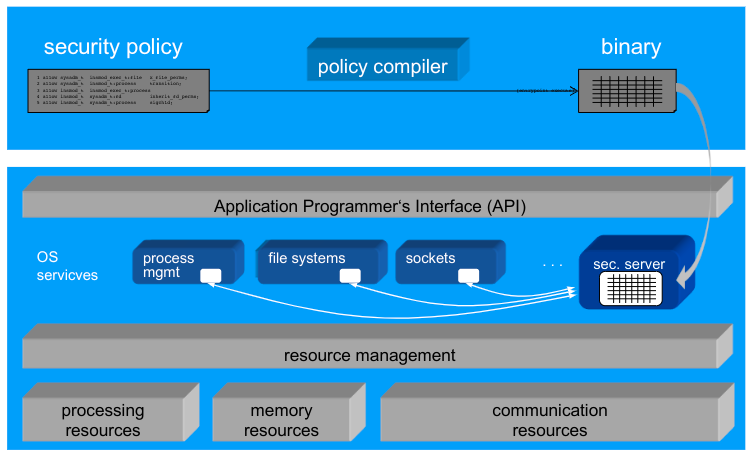
\includegraphics[width=\linewidth]{Assets/Systemsicherheit-fundamental-flask.png}

    Basic Language Concepts
    \begin{itemize*}
        \item Definition of types (a.k.a. ,,domains'')
        \item Labeling of subjects (e.g. processes) with ,,domains'' $\rightarrow passwd_t$
        \item Labeling of objects (e.g. files, sockets) with ,,types'' $\rightarrow shadow_t$
        \item AC: defined by permissions between pairs of types
        \item Dynamic interactions: transitions between domains
    \end{itemize*}

    Policy Rules
    \begin{itemize*}
        \item Grant permissions: allow rules
        \item Typical domains: $user_t$, $bin_t$, $passwd_t$, $insmod_t$, $tomCat_t$, \dots
        \item Classes: OS abstractions (process, file, socket, \dots)
        \item Permissions: read, write, execute, getattr, signal, transition, \dots
    \end{itemize*}

    The Model Behind: 3 Mappings
    \begin{itemize*}
        \item Classification $cl : S\cup O \rightarrow$ C where C $=\{process, file, dir, \dots \}$
        \item Types $type: S\cup O \rightarrow$ T where T $=\{ user_t , passwd_t , bin_t , \dots \}$
        \item Access Control Function (Type Enforcement) $te : T\times T \times C \rightarrow 2^R$
        \item $\rightarrow ACM : T\times( T \times C ) \rightarrow 2^R$
    \end{itemize*}

    \paragraph{Idea only: SELinux RBAC}
    Users and Roles
    \begin{itemize*}
        \item User ID assigned on login
        \item RBAC rules confine type associations ,,Only users in role $doctor_r$ may transit to domain $edit-epr_t$''
        \item[$\rightarrow$] fine-grained domain transitions
        \item[$\rightarrow$] Attributes in SELinux-style RBAC: User ID, Role ID
        \item Specification $\rightarrow$ Tool $\rightarrow$ Binary $\rightarrow$ Security Server
    \end{itemize*}

    Model abstractions
    \begin{itemize*}
        \item TE: MAC rules based on types
        \item ABAC:MAC rules based on attributes
        \item RBAC: MAC rules based on roles
        \item Additionally: BLP-style MLS
    \end{itemize*}

    Other Policy Specification Languages
    \begin{itemize*}
        \item XACML ( eXtensibleAccess Control Markup Language )
        \item NGAC ( Next Generation Access Control Language )
        \item SEAL (Label-based AC policies)
        \item Ponder (Event-based condition/action rules)
        \item GrapPS (Graphical Policy Specification Language)
        \item GemRBAC (Role-based AC models)
        \item PTaCL (Policy re-use by composition)
    \end{itemize*}

    \section{Security Mechanisms}
    Security Models Implicitly Assume
    \begin{itemize*}
        \item Integrity of model implementation
        \begin{itemize*}
            \item Model state
            \item Authorization scheme
        \end{itemize*}
        \item Integrity of model operations call
        \begin{itemize*}
            \item Parameters of authorization scheme ops
            \item Completeness and total mediation of their invocation
        \end{itemize*}
        \item AC, IF: no covert chanels
        \item NI: Rigorous domain isolation
        \item[$\rightarrow$] job of the ,,Trusted Computing Base'' (TCB) of an IT system
    \end{itemize*}

    \note{Trusted Computing Base (TCB)}{The set of functions of an IT system that are necessary and sufficient for implementing its security properties $\rightarrow$ Isolation, Policy Enforcement, Authentication \dots }

    \note{Security Architecture}{The part of a system’s architecture that implement its TCB $\rightarrow$ Security policies, Security Server (PDP) and PEPs, authentication components, \dots }

    \note{Security Mechanisms}{Algorithms and data structures for implementing functions of a TCB $\rightarrow$ Isolation mechanisms, communication mechanisms, authentication mechanisms, \dots }

    $\rightarrow$ TCB - runtime environment for security policies

    \begin{itemize*}
        \item (some) TCB functions are integrated in today's commodity OSes
        \begin{itemize*}
            \item Isolation
            \item Subject/object authentication
        \end{itemize*}
        \item Complex models additionally require implementation of
        \begin{itemize*}
            \item Authorization schemes
            \item Roles, lattices, attributes
            \item[$\rightarrow$] stronger concepts and mechanisms
            \item OS level: Security Server (SELinux, OpenSolaris)
            \item Middleware level: Policy Objects (CORBA, DBMSs)
            \item Application level: user level reference monitors (Flume), user level policy servers (SELinux)
        \end{itemize*}
    \end{itemize*}

    Security mechanisms: A Visit in the Zoo: \dots
    \begin{itemize*}
        \item In OSes
        \begin{itemize*}
            \item Authenticity
            \begin{itemize*}
                \item Of subjects: login
                \item Of objects: object management, e.g. file systems
            \end{itemize*}
            \item Confidentiality and integrity: Access control lists
        \end{itemize*}
        \item In middleware layer (DBMSs, distributed systems)
        \begin{itemize*}
            \item Authentication server (Kerberos AS) or protocols (LDAP)
            \item Authorization: Ticket server (Kerberos TGS)
        \end{itemize*}
        \item In libraries and utilities
        \begin{itemize*}
            \item Confidentiality, integrity, authenticity
            \begin{itemize*}
                \item Cryptographic algorithms
                \item Certificate management for PKIs
                \item Isolation (Sandboxing)
            \end{itemize*}
        \end{itemize*}
    \end{itemize*}

    \subsection{Authorization}
    Lampson, HRU, RBAC, ABAC, BLP, CW $\rightarrow$ ACMs

    \subsubsection{Access Control Lists und Capability Lists}
    Lampson’s ACM: Sets $S$, $O$, $R$ and ACM $m: S\times O\rightarrow 2^R$
    %  | m  | o_1 | o_2  | o_3  | \dots  | o_m |
    %  | --- | --- | ----- | ----- | --- | --- |
    %  | s_1 |
    %  | s_2 |   |    | {r,w} |
    %  | s_3 |   | {r,w} |
    %  | \dots  |   |    |    |   | {w} |
    %  | s_n |

    Properties of an ACM
    \begin{itemize*}
        \item Large (e.g. ,,normal'' file server: $|m| >> 1$ TByte)
        \item Sparsely populated
        \item Subject and object identifications in OSes generally are
        \begin{itemize*}
            \item Not numerical
            \item Not consecutive
        \end{itemize*}
        \item Rows and columns are created and destroyed dynamically
    \end{itemize*}

    Idea: Distributed ACM Implementation
    \begin{enumerate*}
        \item Split matrix into vectors; Column/Row vectors
        \item Attach vectors to subjects resp. objects
    \end{enumerate*}
    \begin{itemize*}
        \item Column vectors
        \begin{itemize*}
            \item Describe every existing right wrt. an object
            \item vector associated to object, part of object‘s metadata
            \item[$\rightarrow$] Access control lists (ACLs)
        \end{itemize*}
        \item Row vectors
        \begin{itemize*}
            \item Describe every existing right wrt. a subject
            \item Associated to its subject, part of subject‘s metadata
            \item[$\rightarrow$] capability lists
        \end{itemize*}
    \end{itemize*}

    ACLs
    \begin{itemize*}
        \item Associated to exactly one object
        \item Describes every existing right wrt. object by a set of tuples
        \item Implemented e.g. as list, table, bitmap
        \item Part of object‘s metadata (generally located in inode)
    \end{itemize*}

    Create and Delete an ACL
    \begin{itemize*}
        \item Together with creation and deletion of an object
        \item Initial rights are create operation parameters $\rightarrow$ discretionary access control
        \item Initial rights issued by third party$\rightarrow$ mandatory access control
    \end{itemize*}

    Modify an ACL
    \begin{itemize*}
        \item Add or remove tuples (subject identification, right set)
        \item Owner has right to modify ACL $\rightarrow$ discretionary access control
        \item Third party has right to modify ACL $\rightarrow$ mandatory access control
        \item Right to modify ACL is part of ACL $\rightarrow$ universal
    \end{itemize*}

    Check Rights
    \begin{itemize*}
        \item Whenever an object is accessed
        \item Search granting tuple in ACL
    \end{itemize*}

    Negative Rights
    \begin{itemize*}
        \item Dominate positive rights
        \item represented by tuples (subject identification, negative rights set)
        \item Rights of subject: difference of positive and negative rights
    \end{itemize*}

    \begin{multicols}{2}
        Example: ACLs in Unix
        \begin{itemize*}
            \item 3 elements per list list
            \item 3 elements per right set
            \item[$\rightarrow$] 9 bits coded in 16-bit-word (PDP 11, 1972)
        \end{itemize*}
        \columnbreak

        \begin{tabular}{c | c | c| c}
                   & read & write & exec \\\hline
            owner  & y    & y     & n    \\
            group  & y    & n     & n    \\
            others & n    & n     & n
        \end{tabular}
    \end{multicols}

    \paragraph{Operations on Capability Lists}
    Create and Delete
    \begin{itemize*}
        \item Together with creation and deletion of a subject
        \item Initial rights same as parent $\rightarrow$ inherited
        \item Constraints by
        \begin{itemize*}
            \item Parent $\rightarrow$ discretionary access control
            \item Capability $\rightarrow$ mandatory access control
        \end{itemize*}
    \end{itemize*}

    Modification: Add or remove tuples (object identification, right set)

    Passing on Capabilities, options:
    \begin{itemize*}
        \item Emission and call-back by capability owner $\rightarrow$ discretionary access control
        \item Emission and call-back by third party $\rightarrow$ mandatory access control
        \item Emission and call-back controlled by capability itself $\rightarrow$ universal
    \end{itemize*}

    \paragraph{$\delta s$ in Administration}
    ACLs: Located near objects $\rightarrow$ finding all rights of a subject expensive

    Example BLP: re-classification of a subject $\rightarrow$ update every ACL with rights of this subject

    Group models; e.g.
    \begin{itemize*}
        \item BLP: subjects with same classification
        \item Unix: subjects belonging to project staff
    \end{itemize*}

    Role models (role: set of rights); e.g. set of rights wrt. objects with same classification

    \paragraph{$\delta s$ in Distributed Systems}
    \begin{itemize*}
        \item No encapsulation of subject ids/ACLs in single trustworthy OS
        \item No encapsulation of cap. lists in a single trustworthy OS kernel
        \begin{itemize*}
            \item Authentication and management on subject’s system
            \item Transfer via open communication system
            \item Checking of capabilities and subject ids on object’s system
        \end{itemize*}
    \end{itemize*}

    Vulnerabilities and Counteractions
    \begin{itemize*}
        \item Subject’s system may fake subject ids
        \item Consequence: Reliable subject authentication required $\rightarrow$ authentication architectures (e.g. Kerberos)
        \item Non-trustworthy subject systems modify capabilities
        \begin{itemize*}
            \item[$\rightarrow$] cryptographic sealing of capabilities such that
            \item Issuer can be determined
            \item Modification can be detected
            \item sealing e.g. by digital signatures
        \end{itemize*}
        \item Non-trustworthy subject systems pass capabilities to third parties or are copied by third parties while in transit $\rightarrow$ personalized
        \item Exploit stolen capabilities by forging subject id
        \begin{itemize*}
            \item[$\rightarrow$] cryptographically sealed personalized capabilities
            \item[$\rightarrow$] reliable subject authentication required
            \item[$\rightarrow$] authentication architectures
        \end{itemize*}
    \end{itemize*}

    \paragraph{Expressive Power of ACLs and Capability Lists}
    \begin{itemize*}
        \item Efficient data structures for implementing ACMs/ACFs
        \item Located in OSs, middleware, DBMSe, application systems
        \item Correctness, tamperproofness, total S/O interaction mediation vital for enforcing access control $\rightarrow$ implementation by strong architectural principles
        \item Assume reliable authentication of subjects and objects $\rightarrow$ support by further security mechanisms
        \item Are too weak to implement complex security policies
        \item Not sufficient for implementing more complex security policies $\rightarrow$ Authorization schemes
    \end{itemize*}

    \subsubsection{Interceptors}
    Policy implementation by algorithms instead of lists
    \begin{itemize*}
        \item Tamperproof runtime environments for security policies
        \item In total control of subject/object interactions (Observation, Modification, Prevention)
    \end{itemize*}

    General Architectural Principle: Separation of
    \begin{itemize*}
        \item (Replaceable) strategies
        \item (Strategy-independent) mechanisms
    \end{itemize*}

    Applied to Interceptors $\rightarrow$ 2 Parts
    \begin{itemize*}
        \item Runtime environment for security policies (strategies)
        \begin{itemize*}
            \item often called ,,policy decision point'' (PDP)
        \end{itemize*}
        \item Interception points (mechanisms)
        \begin{itemize*}
            \item often called ,,policy enforcement points'' (PEP)
        \end{itemize*}
    \end{itemize*}

    Summary
    \begin{itemize*}
        \item RTE for security policies in policy-controlled systems
        \begin{itemize*}
            \item SELinux: ,,Policy Server''
            \item CORBA: ,,Policy Objects''
        \end{itemize*}
        \item Architecture: separation of responsibilities
        \item Strategic component State and authorization scheme
        \item Policy enforcement: total policy entities interaction mediation
        \item Generality: implement a broad scope of policies (computable)
        \begin{itemize*}
            \item[$\rightarrow$] rules based on checking digital signatures
            \item[$\rightarrow$] interceptor checks/implements encryption
        \end{itemize*}
    \end{itemize*}

    \subsection{Cryptographic Security Mechanisms}
    Encryption: Transformation of a plaintext into a ciphertext
    \begin{itemize*}
        \item 2 functions encrypt, decrypt
        \item 2 keys k1, k2
        \item $text = decrypt_{k2}(encrypt_{k1}(text))$ or simply
        \item $text = \{\{text\}_{k1}\}_{k2}$ (if encryption function is obvious)
        \item Symmetric schemes (secret key): one single key: $k1=k2$
        \item Asymmetric schemes (public key): two different keys: $K1\not=K2$
    \end{itemize*}

    \paragraph{Kerkhoff’s Principle}
    \begin{enumerate*}
        \item Encryption functions (algorithms) are publicly known
        \begin{itemize*}
            \item[$\rightarrow$] many experts look at it
            \item[$\rightarrow$] quality advantage assumed
        \end{itemize*}
        \item Keys are secret
        \begin{itemize*}
            \item[$\rightarrow$] encryption security depends on
            \item Properties of algorithms
            \item Confidentiality of keys
        \end{itemize*}
    \end{enumerate*}

    \paragraph{Symmetric Encryption Schemes}
    \begin{itemize*}
        \item Encryption and decryption with same key
        \item[$\rightarrow$] security based on keeping key secret
        \item Example: shift letters of a ciphertext forward by K positions
    \end{itemize*}

    Application Examples
    \begin{enumerate*}
        \item Confidentiality of Communication (Assumptions)
        \begin{itemize*}
            \item Sender and receiver share key k , which has to be established before communication, Authentically, Confidentially
            \item Nobody else must know $k(secretkey)$
        \end{itemize*}
        \item Authentication: client to server (by shared secret key)
        \begin{itemize*}
            \item Each client shares an individual and secret key $k_{client}$ with server
            \item Server and clients keep key secret
            \item Server reliably generates a nonce (=never sent once before )
        \end{itemize*}
        \item Sealing of Documents, e.g. Capabilities
        \begin{itemize*}
            \item 1 key owner $\rightarrow$ owner may
            \begin{itemize*}
                \item seal document
                \item check whether seal is sound
            \end{itemize*}
            \item Group of key owners $\rightarrow$ each group membermay
            \begin{itemize*}
                \item Seal document
                \item Check whether seal was impressed by group member
                \item[$\rightarrow$] nobody in this group can prove it was him or not
            \end{itemize*}
            \item Outside the group $\rightarrow$ nobody can do any of these things
        \end{itemize*}
    \end{enumerate*}

    Algorithms: Block and Stream Ciphers
    \begin{itemize*}
        \item Block cipher
        \begin{itemize*}
            \item Decompose plaintext into blocks of equal size (e.g. 64 bits)
            \item Encrypt each block
            \item e.g. Data Encryption Standard (DES) obsolete since 1998
            \item e.g. Advanced Encryption Standard (AES) (128bits length)
        \end{itemize*}
        \item Stream cipher
        \begin{itemize*}
            \item Encrypt each digit of a plaintext stream by a cipher digit stream (e.g. by XOR)
            \item Cipher digit stream: pseudo-random digit stream
        \end{itemize*}
    \end{itemize*}

    \paragraph{Asymmetric Encryption Schemes}
    \begin{itemize*}
        \item[$\rightarrow$] key pair $(k1,k2) = (k_{pub} , k_{sec})$ where
        \item $decrypt_{k_{sec}} ( encrypt_{k_{pub}} (text)) = text$
        \item Conditio sine qua non: Secret key not computable from public key
    \end{itemize*}

    Application Examples
    \begin{enumerate*}
        \item Confidentiality of Communication (compare symmetric encryption schemes)
        \begin{itemize*}
            \item Sender shares no secret with receiver $\rightarrow$ No trust between sender and receiver necessary
            \item Sender must know public key of receiver $\rightarrow$ public-key-Infrastructures (PKIs) containing key certificates
        \end{itemize*}
        \item Authentication: using public key
        \begin{itemize*}
            \item Each client owns an individual key pair ($k_{pub}, k_{sec}$)
            \item Server knows public keys of clients (PKI)
            \item Clients are not disclosing secret key
            \item Server reliably generates nonces
            \item Properties
            \begin{itemize*}
                \item Client and server share no secrets
                \item No key exchange before communication
                \item No mutual trust required
                \item But: sender must know public key of receiver
                \item[$\rightarrow$] PKIs
            \end{itemize*}
        \end{itemize*}
        \item Sealing of Documents, compare sealing using secret keys
        \begin{itemize*}
            \item $\exists$ just 1 owner of secret key $\rightarrow$ only she may seal contract
            \item Knowing her public key,
            \begin{itemize*}
                \item[$\rightarrow$] everybody can check contract’s authenticity
                \item[$\rightarrow$] everybody can prove that she was the sealer
                \item[$\rightarrow$] repudiability: digital signatures
            \end{itemize*}
        \end{itemize*}
    \end{enumerate*}

    Consequence of Symmetric vs. Asymmetric Encryption
    \begin{itemize*}
        \item[Sym] shared key, integrity and authenticity can be checked only by key holders $\rightarrow$ message authentication codes (MACs)
        \item[Asym] integrity and authenticity can be checked by anyone holding public key (only holder of secret key could have encrypted the checksum) $\rightarrow$ digital signatures
    \end{itemize*}

    Key Distribution for Symmetric Schemes
    \begin{itemize*}
        \item Asymmetric encryption is expensive
        \item Key pairs generation (High computational costs, trust needed)
        \item Public Key Infrastructures needed for publishing public keys
        \item[$\rightarrow$] Use asymmetric key for establishing communication
        \item Use symmetric encryption for communication
    \end{itemize*}

    \paragraph{RSA Cryptosystem (Rivest/Shamir/Adleman)}
    Attractive because $encrypt=decrypt$ $\rightarrow$ universal:
    \begin{enumerate*}
        \item Confidentiality
        \item Integrity and authenticity (non repudiability, digital signatures)
    \end{enumerate*}
    For $n\in\mathbb{N}$ we search 2 primes $p$ and $q$ such that $n=p*q$
    \begin{itemize*}
        \item[$\rightarrow$] hard problem because for factorization, prime numbers are needed
        \item There are many of them, approx. $7*10^{151}$
        \item Finding them is extremely expensive: Sieve of Eratosthenes
        \item Optimization: Atkin’s Sieve, $O(n^{1/2+O(1)})$
        \item Until today, no polynomial factorization algorithm is known
        \item Until today, nobody proved that such algorithm cannot exist\dots
    \end{itemize*}
    Precautions in PKIs: Prepare for fast exchange of cryptosystem

    \subsubsection{Cryptographic Hash Functions}
    Discover violation of integrity of data, so that integrity of information is maintained.
    \begin{itemize*}
        \item Checksum generation by cryptographic hash functions
        \item Checksum encryption
        \item Integrity check by
        \begin{itemize*}
            \item Generating a new checksum
            \item Decryption of encrypted checksum
            \item Comparison of both values
        \end{itemize*}
    \end{itemize*}

    Method of Operation: Map data of arbitrary length to checksum of fixed length such that $Text1 \not= Text2 \Rightarrow hash(Text1) \not= hash(Text2)$ with high probability

    \begin{itemize*}
        \item 160 - Bit checksums: RIPEMD-160 (obsolete since 2015)
        \item Secure Hash Algorithm (SHA-1, published NIST 1993)
        \item Larger Checksums: SHA-256, SHA-384, SHA-512
        \item 128-Bit: Message Digest (MD5 (1992)) (no longer approved)
        \item MD5: belongs to IPsec algorithm group, used also in SSL
    \end{itemize*}

    \subsubsection{Digital Signatures}
    \begin{itemize*}
        \item assert author of a document (signer) $\rightarrow$ Authenticity
        \item discover modifications after signing $\rightarrow$ Integrity $\rightarrow$ non repudiability
    \end{itemize*}

    Approach
    \begin{itemize*}
        \item Create signature
        \begin{itemize*}
            \item Integrity: create checksum $\rightarrow$ cryptographic hash function
            \item Authenticity: encrypt checksum $\rightarrow$ use private key of signer
        \end{itemize*}
        \item Check signature
        \begin{itemize*}
            \item Decrypt checksum using public key of signer
            \item Compare result with newly created checksum
        \end{itemize*}
    \end{itemize*}

    \subsubsection{Cryptographic Attacks}
    \paragraph{Ciphertext Only Attacks (weakest assumptions)}
    \begin{itemize*}
        \item Known: ciphertext $CT$
        \item Wanted: plaintext $T$, $Ke$, $Kd$, algorithm
        \item Typical assumptions
        \begin{itemize*}
            \item $CT$ was completely generated by one $Ke$
            \item Known algorithm
            \item Observation of packet sequences in networks
            \item Listening into password-based authentication
        \end{itemize*}
    \end{itemize*}

    \paragraph{Known Plaintext Attacks}
    \begin{itemize*}
        \item Known: $T$ and $CT$ (respectively parts thereof)
        \item Wanted: $Ke$, $Kd$, algorithm
        \item Listening into challenge/response protocols
        \begin{itemize*}
            \item Server $\rightarrow$ Client: nonce
            \item Client $\rightarrow$ Server: $\{nonce\}_{Ke}$
        \end{itemize*}
        \item countermeasure often: Client $\rightarrow$ Server:$\{nonce + Time\}_{Ke}$
    \end{itemize*}

    \paragraph{Chosen Plaintext Attacks}
    \begin{itemize*}
        \item Known: $T$ and $CT$ where $T$ can be chosen by attacker
        \item Wanted: $Ke, Kd$ (algorithm often known)
        \item Authentication in challenge/response protocols
        \begin{itemize*}
            \item Attacker (malicious server) tries to find client’s private key
            \item sends tailored nonces
        \end{itemize*}
        \item Authentication by chosen passwords
        \begin{itemize*}
            \item Attacker tries to find login password
            \item Generates passwords \& compare encryptions with pw DB
        \end{itemize*}
    \end{itemize*}

    \paragraph{Chosen Ciphertext Attacks}
    \begin{itemize*}
        \item Known: $T,CT$ and $Kd$, $CT$ can be chosen, $T$ can be computed
        \item wanted: $Ke$ $\rightarrow$ successful attacks allow forging digital signatures
        \item Attack by
        \begin{itemize*}
            \item (within limits) Servers while authenticating clients
            \item (within limits) Observers of such authentications
            \item In a PK cryptosystem: Everybody knowing $Kd$
        \end{itemize*}
    \end{itemize*}

    Goals of Cryptographic Algorithms
    \begin{itemize*}
        \item To provide security properties such as
        \begin{itemize*}
            \item Integrity, confidentiality, non-repudiability
            \item Of communication
            \item Of resources such as files, documents, program code
        \end{itemize*}
        \item Especially: implement assumptions made by security models like
        \begin{itemize*}
            \item Authenticity, integrity, confidentiality of
            \item Model entities (subjects, objects, roles, attributes)
            \item Model implementations
        \end{itemize*}
    \end{itemize*}

    Beware: Many Pitfalls!
    \begin{itemize*}
        \item Weaknesses of mathematical foundations $\rightarrow$ unproved assumptions
        \item Weaknesses of algorithms $\rightarrow$ cryptographic attacks
        \item Weaknesses of key generation $\rightarrow$ e.g. weak prime numbers
        \item Weaknesses of mechanism use $\rightarrow$ co-existence of mechanisms
    \end{itemize*}

    \subsection{Identification and Authentication}
    To reliably identify people, systems,\dots.

    Approaches: Proof of identity by
    \begin{itemize*}
        \item By proving knowledge of simple secret $\rightarrow$ passwords
        \item By biophysicproperties $\rightarrow$ biometrics
        \item By proving knowledge of simple secret $\rightarrow$ cryptographic protocols
    \end{itemize*}

    \subsubsection{Passwords}
    \begin{itemize*}
        \item Used For: Authentication of humans to IT systems
        \item Verified Item: Knowledge of simple secret
        \item Convenient
        \item Easy to guess / compute (RainbowCrack: $104*10^9$ hash/second)
        \begin{itemize*}
            \item[$\rightarrow$] password generators
            \item[$\rightarrow$] password checkers (min. 8 chars, \dots )
        \end{itemize*}
        \item Problem of careless handling (password on post-it)
        \item Input can easily be observed (see EC PINs)
        \item[$\rightarrow$] Confidential communication with authenticating system
    \end{itemize*}

    \subsubsection{Biometrics}
    \begin{itemize*}
        \item Used For: Authentication of humans to IT systems
        \item Verified Items: Individual properties like voice, hand/retina, finger
        \item Verification: By comparing probe with reference pattern
        \item Pros: (prospectively) Difficult to counterfeit
        \begin{itemize*}
            \item Convenient, no secrets to remember, cannot be lost
            \item Difficult to intentionally pass on
        \end{itemize*}
        \item Contras: Fundamental technical problems
        \begin{itemize*}
            \item Comparison methods with reference fuzzy techniques
            \item False Non-match Rate: authorized people are rejected
            \item False Match Rate: not authorized people are accepted
            \item Susceptible environmental conditions (noise, dirt, fractured)
            \item Social Barriers, Acceptance
        \end{itemize*}
        \item Fundamental weaknesses in distributed systems $\rightarrow$ Secure communication to authenticating system required (personal data)
        \item Reference probes are personal data $\rightarrow$ Data Protection Act
        \item Reaction time on security incidents $\rightarrow$ Passwords, smartcards can be exchanged easily
    \end{itemize*}

    \subsubsection{Cryptographic Protocols}
    \paragraph{SmartCards}
    \begin{itemize*}
        \item Used For: Authentication of humans to IT systems
        \item Verified Item: Knowledge of complex secret
        \begin{itemize*}
            \item Secret part of asymmetric key pair
            \item Symmetric key
        \end{itemize*}
        \item Verification
        \begin{itemize*}
            \item Challenge/response protocols
            \item Goal: Proof that secret is known
            \item Contrary to password authentication, no secret exposure
        \end{itemize*}
    \end{itemize*}

    Vehicle for Humans: SmartCards
    \begin{itemize*}
        \item Small Computing Devices encompassing Processor(s), RAM, Persistent memory, Communication interfaces
        \item What They Do
        \begin{itemize*}
            \item Store and keep complex secrets (keys)
            \item Run cryptographic algorithms
            \begin{itemize*}
                \item Response to challenges in challenge/response protocols
                \item Encrypt incoming nonces
            \end{itemize*}
            \item Launch challenges to authenticate other principals
            \begin{itemize*}
                \item Generate nonces, verify response
            \end{itemize*}
        \end{itemize*}
    \end{itemize*}

    Properties
    \begin{itemize*}
        \item no secret is exposed
        \begin{itemize*}
            \item[$\rightarrow$] no trust in authenticating system required
            \item[$\rightarrow$] no trust in network required
        \end{itemize*}
        \item Besides authentication other features possible $\rightarrow$ digital signatures, credit card, parking card \dots
        \item Weak verification of card right to use card (PIN, password) $\rightarrow$ some cards have finger print readers
        \item Power supply for contactless cards
    \end{itemize*}

    \paragraph{Authentication Protocols}
    \begin{itemize*}
        \item Used For: Authentication between IT systems
        \item Method: challenge/response-scheme
        \item Based on symmetric \& asymmetric key
    \end{itemize*}
    The 2 fundamental Scenarios
    \begin{enumerate*}
        \item After one single authentication, Alice wants to use all servers in a distributed system of an organization.
        \item Alice wants authentic and confidential communication with Bob. Authentication Server serves session keys to Bob and Alice
    \end{enumerate*}

    Needham-Schroeder Authentication Protocol (for secret keys)
    \begin{itemize*}
        \item establish authentic and confidential communication between 2
        \item[$\rightarrow$] confidentiality, integrity, authenticity
    \end{itemize*}
    \begin{enumerate*}
        \item Authentication of Alice to Bob $\rightarrow$ Bob knows other end is Alice
        \item Authentication of Bob to Alice $\rightarrow$ Alice knows other end is Bob
        \item Establish fresh secret: a shared symmetric session key
    \end{enumerate*}

    Fundamental
    \begin{itemize*}
        \item Common trust in same authentication server
        \item Client-specific secret keys ($K_{AS}, K_{BS}$)
    \end{itemize*}

    %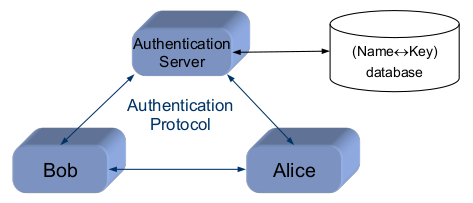
\includegraphics[width=\linewidth]{Assets/Systemsicherheit-needham-schreoeder.png}
    %Note: Protocol used in Kerberos security architecture

    Message Semantics
    \begin{enumerate*}
        \item $A\rightarrow S:A,B,N_A$: A requests session key for B from S
        \item $S\rightarrow A:\{N_A,B,K_{AB},K_{AB},A\}_{KBS}\}_{KAS}$: S responds encrypted with $K_{AS}$ such that only A is able to understand
        \begin{itemize*}
            \item nonce proves that 2. is a reply to 1. (fresh)
            \item session key $K_{AB}$
            \item ticket for B; encryption proves $K_{AB}$ was generated by $S$
        \end{itemize*}
        \item $A\rightarrow B:\{K_{AB},A\}_{KBS}$: A ticket to B; encryption as challenge
        \item $B\rightarrow A:\{N_B\}_{KAB}$: B decrypts ticket \& verifies if A knows $K_{AB}$
        \item $A\rightarrow B:\{N_B-1\}_{KAB}$: A proves by using $K_{AB}$ that he was the sender of 3. (response)
        \begin{itemize*}
            \item Authentication of A to B: only A can decrypt 2.
            \item Authentication of B to A: only B can decrypt 3.
            \item A and B now also share a secret session key
        \end{itemize*}
    \end{enumerate*}

    Authentication Servers
    \begin{itemize*}
        \item Common trust in server by all principals $\rightarrow$ closed user group
        \item Server shares individual secret with each principal (sym key)
    \end{itemize*}

    Needham-Schroeder Authentication Protocol for public keys
    \begin{itemize*}
        \item establish authentic and confidential communication between Principals
        \item Premise: Trust
        \begin{itemize*}
            \item Individually in issuer of certificate (certification authority)
            \item[$\rightarrow$] much weaker than secret key based authentication
        \end{itemize*}
        \item Message Semantics
        \begin{enumerate*}
            \item $A\rightarrow S:A,B$: A requests public key of B
            \item $S\rightarrow A:\{PK_B,B\}_{SK_S}$: S sends certificate; A knows public key of CA
            \item $A\rightarrow B:\{N_A,A\}_{PK_B}$: A sends challenge to B
            \item $B\rightarrow S:B,A$: B requests public key of A
            \item $S\rightarrow B:\{PK_A,A\}_{SK_S}$: S responds (see 2.)
            \item $B\rightarrow A:\{N_A, N_B\}_{PK_A}$: B proves it is B and challenges A
            \item $A\rightarrow B:\{N_B\}_{PK_B}$: A replies and proves it is A
        \end{enumerate*}
        \begin{itemize*}
            \item Authentication of A to B: 6. together with 7.
            \item Authentication of B to A: 3. together with 6.
            \item From where key certificates are obtained is irrelevant
        \end{itemize*}
    \end{itemize*}

    Certificate Servers: Basis of Authentication
    \begin{itemize*}
        \item Key certificates
        \begin{itemize*}
            \item Digitally signed mappings (name $\leftrightarrow$ public key)
            \item Issued by certification authorities (CA)
        \end{itemize*}
        \item Certificate servers
        \begin{itemize*}
            \item Manage certificate data base
            \item Need not be trustworthy
        \end{itemize*}
    \end{itemize*}
    %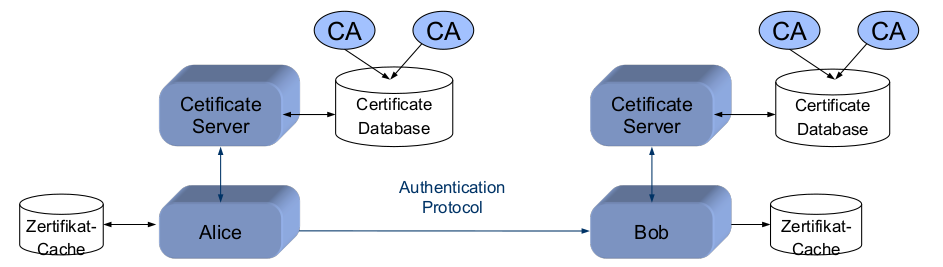
\includegraphics[width=\linewidth]{Assets/Systemsicherheit-Certificate-server.png}

    $\delta s$ between Secret Key and Public Key Authentication
    \begin{itemize*}
        \item Secret Key Authentication
        \begin{itemize*}
            \item Requires common trust in AS, a-priori key exchange and mutual trust in keeping session key secret
            \item Allows for message authentication codes
            \item Require online AS
            \item accumulation of secrets at AS $\rightarrow$ dangerous, server always online
            \item n keys for authenticating n principals
            \item $O(n^2)$ session keys for n communicating parties
        \end{itemize*}
        \item Public Key Authentication
        \begin{itemize*}
            \item Requires knowledge of public keys $\rightarrow$ PKIs
            \item Allows for digital signatures
            \item Allow for local chaching of certificates
            \item n keys for authenticating n principals
            \item $O(n)$ keys for $n$ communicating parties if PKs are used
            \item $O(n^2)$ key for n comm. parties if session keys are used
            \item Certificate management: PKIs, CAs, data bases, \dots
        \end{itemize*}
    \end{itemize*}

    \section{Security Architectures}
    Security architectures have been around for a long time \dots
    \begin{itemize*}
        \item Architecture Components (Buildings, walls, windows,\dots )
        \item Architecture (Component arrangement and interaction)
        \item Build a stronghold such that security policies can be enforced
        \begin{itemize*}
            \item Presence of necessary components/mechanisms
            \item Totality of interaction control (,,mediation'')
            \item Tamperproofness
            \item[$\rightarrow$] architecture design principles
        \end{itemize*}
    \end{itemize*}

    Check your trust in
    \begin{itemize*}
        \item Completeness of access mediation (and its verification!)
        \item Policy tamperproofness(and its verification!)
        \item TCB correctness (and its verification!)
    \end{itemize*}

    Problem Areas PDPs/PEPs are
    \begin{itemize*}
        \item Scattered among many OS components $\rightarrow$ Problem of architecture
        \item Not robust
        \begin{itemize*}
            \item Not isolated from errors within the entire OS
            \item Especially in dynamically loaded OS modules
            \item[$\rightarrow$] Problem of security architecture implementation
        \end{itemize*}
        \item OSes/Middleware/Applications are big
        \item Only a small set of their functions logically belongs to the TCB
        \item[$\rightarrow$] architecture design such that TCB functions are collected
        \begin{itemize*}
            \item not bypassable (total access mediation),
            \item isolated (tamperproofness),
            \item trustworthy (verifiable correctness) core
            \item[$\rightarrow$] architecture such that these properties are enforced
        \end{itemize*}
    \end{itemize*}

    \subsection{Architecture Design Principles}
    Definitions of fundamental security architecture design principles
    \begin{itemize*}
        \item Complete
        \item Tamperproof
        \item Verifiably correct
        \item control of all security-relevant actions in a system
    \end{itemize*}

    \subsubsection{The Reference Monitor Principles}
    There exists an architecture component that is
    \begin{itemize*}
        \item[RM1] Involved in any subject/object interaction $\rightarrow$ total mediation property
        \item[RM2] Well-isolated from the rest of the systems $\rightarrow$ tamperproofness
        \item[RM3] Small and well-structured enough to analyze correctness by formal methods $\rightarrow$ verifiability
    \end{itemize*}

    architecture component built along these: ,,Reference Monitor''
    \begin{itemize*}
        \item 1 PDP (policy implementation)
        \item many PEPs (interceptors, policy enforcement)
    \end{itemize*}

    Reference Monitor
    \begin{itemize*}
        \item Core component of a TCB
        \item Typically encloses
        \begin{itemize*}
            \item Security policy implementation(s) (PDP)
            \begin{itemize*}
                \item Model state (e.g. ACM, subject set, entity attributes)
                \item Model behavioral logic (e.g.authorization scheme)
            \end{itemize*}
            \item Enforcement mechanisms: PEPs
        \end{itemize*}
        \item Typically excludes (due to complexity and size, RM 3)
        \begin{itemize*}
            \item Authentication
            \item Cryptographic mechanisms
            \item Sometimes also model state (e.g.ACLs)
        \end{itemize*}
    \end{itemize*}

    Consequences of (RM 3) for TCBs
    \begin{itemize*}
        \item Few functions $\rightarrow$ small size (LoC)
        \item Simple functions $\rightarrow$ low complexity
        \item Strong isolation
        \item Precisely known perimeter
    \end{itemize*}

    \subsubsection{Implementation Layers}
    \begin{multicols}{2}
        Monolithic OS Kernel 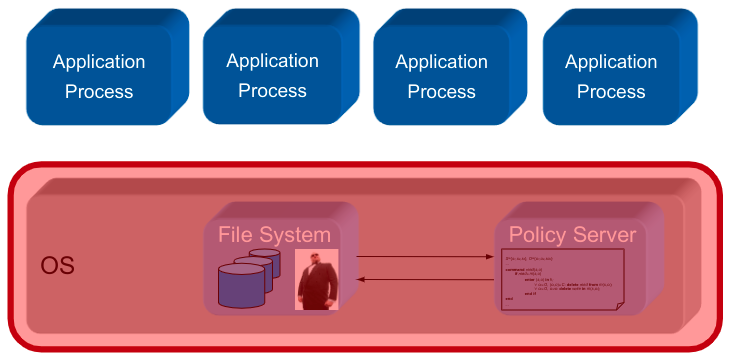
\includegraphics[width=\linewidth]{Assets/Systemsicherheit-policy-controlled-os-tcp-implementation.png}
        \columnbreak

        Microkernel Architecture (Nizza) 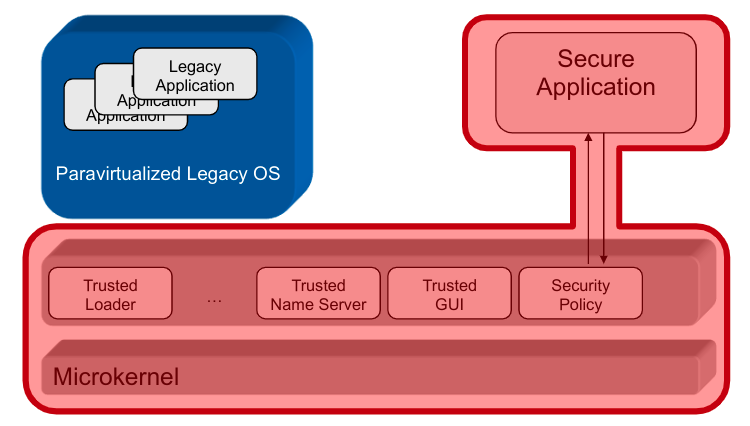
\includegraphics[width=\linewidth]{Assets/Systemsicherheit-policy-microkernel-tcp-functional.png}
    \end{multicols}
    \begin{multicols}{2}
        Middleware-level Policy 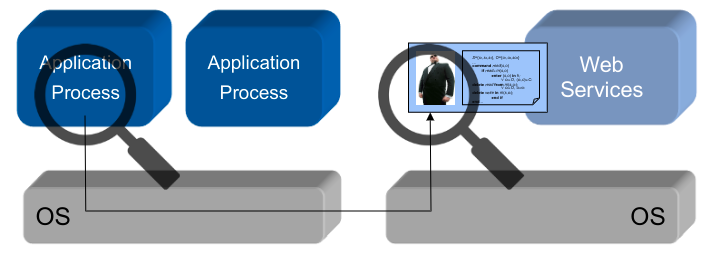
\includegraphics[width=\linewidth]{Assets/Systemsicherheit-middleware-level-policy.png}
        \columnbreak

        Application 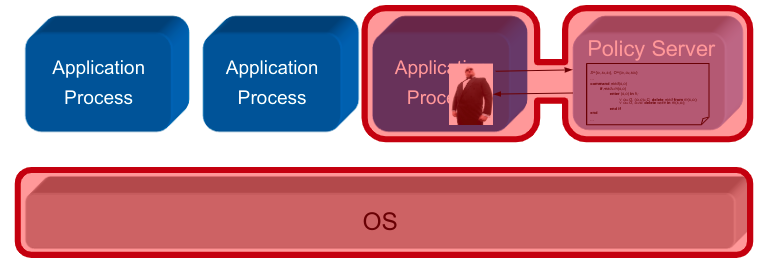
\includegraphics[width=\linewidth]{Assets/Systemsicherheit-policy-controlled-app-tcp-implementation.png}
    \end{multicols}
    \begin{itemize*}
        \item Numerous rather weak implementations in Middleware, Applications\dots
        \item Stronger approaches in Microkernel OSes, Security-focused OS
    \end{itemize*}

    \subsubsection{Nizza}
    \begin{itemize*}
        \item RM1 - RM3 (Especially: Small TCB)
        \item Maintain functionality of
        \begin{itemize*}
            \item Contemporary legacy OSes
            \item Legacy Applications (,,legacy'' = unmodified for security)
        \end{itemize*}
    \end{itemize*}

    Concepts/Reference monitor principles:
    \begin{itemize*}
        \item Separation of OS, Applications into security-critical vs. non-critical components $\rightarrow$ precise identification of (minimal) TCB
        \item Maintain functionality $\rightarrow$ Paravirtualization of standard legacy OS
    \end{itemize*}

    OS View
    %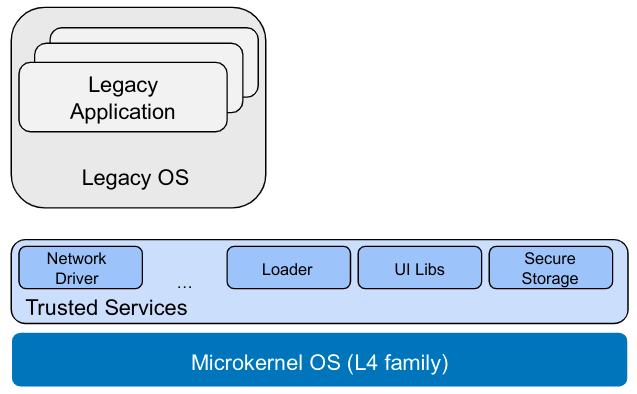
\includegraphics[width=\linewidth]{Assets/Systemsicherheit-nizza-os-view.png}
    \begin{itemize*}
        \item Trustworthy microkernel
        \item Trustworthy basic services
        \item Not trustworthy (paravirtualized) legacy OS
    \end{itemize*}

    Application View
    \begin{itemize*}
        \item Vulnerability increases with growing complexity $\rightarrow$ reduce vulnerability of security-critical code by
        \item Software functionality separation
        \item Isolation of functional domains %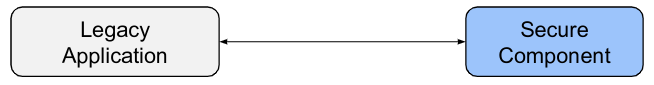
\includegraphics[width=\linewidth]{Assets/Systemsicherheit-nizza-application-view.png}
        \item Example: Email Client
        \begin{itemize*}
            \item Non-critical: reading/composing/sending emails
            \item Critical: signing emails (email-client $\leftrightarrow$ Enigmail Signer)
        \end{itemize*}
    \end{itemize*}

    %Putting it all Together
    %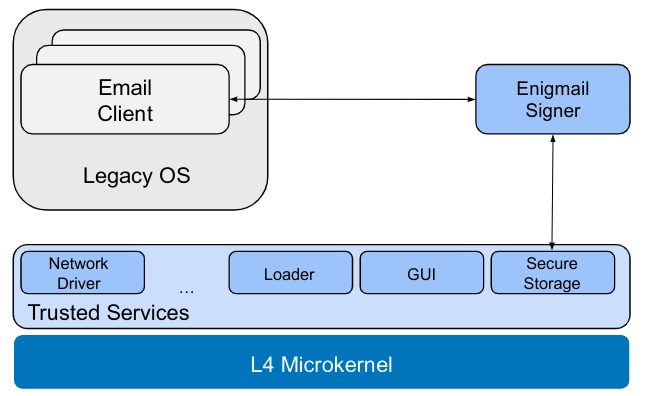
\includegraphics[width=\linewidth]{Assets/Systemsicherheit-nizza-enigmail.png}
    %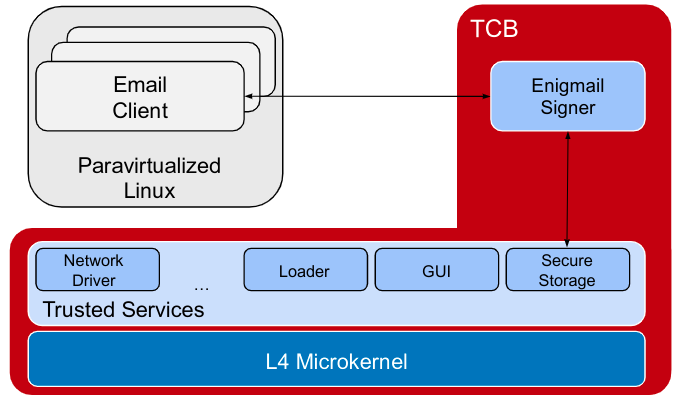
\includegraphics[width=\linewidth]{Assets/Systemsicherheit-nizza-enigmail-tcb.png}

    \begin{itemize*}
        \item Code size of TCB reduced by 2 orders of magnitude
        \item Functionality of legacy OSes and applications preserved
        \item (Moderate) performance penalties
        \item Paravirtualization of legacy OS
        \item Decomposition of trusted applications
    \end{itemize*}

    \subsubsection{Security Enhanced Linux (SELinux)}
    \begin{itemize*}
        \item State-of-the-art OS
        \item State-of-the-art security paradigms
        \item[$\rightarrow$] Policy-controlled (Linux) (Security-aware) OS kernel
    \end{itemize*}

    Security Policies in SELinux
    \begin{itemize*}
        \item Implementation by new OS abstractions
        \item Somewhat comparable to ,,process'' abstraction
        \item Specification of a\dots
        \begin{itemize*}
            \item process is a program: algorithm implemented in formal language
            \item security policy is a security model: rule set in formal language
        \end{itemize*}
        \item Runtime environment (RTE) of a \dots
        \begin{itemize*}
            \item process is OSprocess management $\rightarrow$ RTE for application-level programs
            \item security policy is OS security Server $\rightarrow$ RTE for kernel-level policies
        \end{itemize*}
    \end{itemize*}

    SELinux Architecture
    %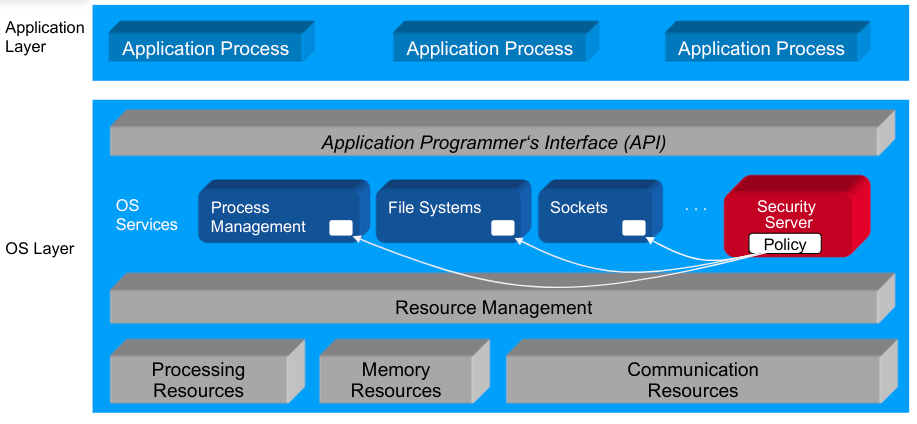
\includegraphics[width=\linewidth]{Assets/Systemsicherheit-selinux-architecture.png}
    \begin{itemize*}
        \item Policy-aware Security Server (policy decision point, PDP) $\rightarrow$ Policy RTE in kernel‘s protection domain
        \item Interceptors (policy enforcement points, PEPs) $\rightarrow$ Total interaction control in object managers
    \end{itemize*}

    Implementation Concepts
    \begin{itemize*}
        \item Reference Monitor Principles
        \begin{itemize*}
            \item Total mediation of security-relevant interactions $\rightarrow$ placement of PEPs: Integration into object managers
            \item Tamperproofness of policy implementation $\rightarrow$ placement of PDP: Integration into kernel
        \end{itemize*}
        \item Policy Support
        \begin{itemize*}
            \item Authenticity of entities: Unique subject/object identifiers
            \item Policy-specific entity attributes (type, role, MLS label)
        \end{itemize*}
        \item Problem in Linux,
        \begin{itemize*}
            \item Subject identifiers (PIDs) or object identifiers (i-node numbers) are
            \begin{itemize*}
                \item neither unique
                \item nor are of uniform type
            \end{itemize*}
            \item[$\rightarrow$] security identifier (SID)
            \item Policy-specific subject/object attributes (type, role) are not part of subject/object metadata $\rightarrow$ security context
            \item[$\rightarrow$] Approach: Extensions of process/file/socket\dots -management
        \end{itemize*}
    \end{itemize*}

    Authenticity of Entities
    \begin{itemize*}
        \item Object managers help: implement injective mapping SEO $\rightarrow$ SID
        \begin{itemize*}
            \item SID created by security server
            \item Mapping of SIDs to objects by object managers
        \end{itemize*}
    \end{itemize*}
    %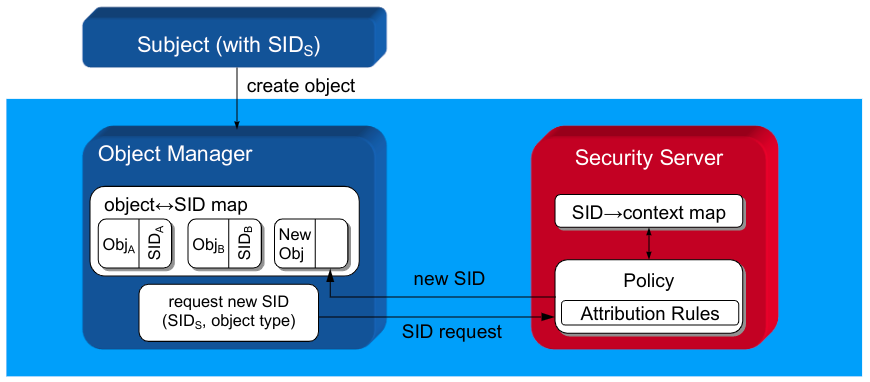
\includegraphics[width=\linewidth]{Assets/Systemsicherheit-object-managers.png}

    Entity Attributes
    \begin{itemize*}
        \item sec. policy implements injective mapping SID $\rightarrow$ security context
        \item sec. contexts creation according to policy-specific labeling rules
        \item Entry in SID $\rightarrow$ security context mapping table
    \end{itemize*}

    Security Context contains
    \begin{itemize*}
        \item Standard entity attributes such as user ID, Role, Type
        \item Policy-specific entity attributes such as Confidentiality/clearance level (e.g. MLS label)
        \item is implemented as a text string with policy-dependent format
    \end{itemize*}

    Problem: Security contexts of persistent Entities
    \begin{itemize*}
        \item Policies not aware of persistency of entities $\rightarrow$ persistency of security contexts is job of object managers
        \item Layout of object metadata is file system standard $\rightarrow$ security contexts cannot be integrated in i-nodes (their implementation: policy-independent)
    \end{itemize*}

    Solution
    \begin{itemize*}
        \item Persistent objects additionally have persistent SID : ,,PSID''
        \item OMs map these to SID
        \item 3 invisible storage areas in persistent memory implementing
        \begin{itemize*}
            \item Security context of file system itself (label)
            \item Bijective mapping: inode $\rightarrow$ PSID
            \item Bijective mapping: PSID $\rightarrow$ security context
        \end{itemize*}
    \end{itemize*}

    Access Vector Cache(AVC)
    \begin{itemize*}
        \item Located in object managers (user level) resp. in Security Server (kernel level)
        \item Caches access decisions
    \end{itemize*}

    RM Evaluation of SELinux
    \begin{itemize*}
        \item Compliance with Reference Monitor Principles
        \item Total Mediation Property (placement of PEPs) done manually
        \item Tamperproofness of Policy Implementation
        \begin{itemize*}
            \item Fundamental problem in monolithic software architectures
            \item[$\rightarrow$] TCB implementation vulnerable from entire OS kernel code
            \item Security server, All object managers, Memory management,\dots
            \item It can be done: Nizza
        \end{itemize*}
        \item Verifiability
        \begin{itemize*}
            \item Size and complexity of policy $\rightarrow$ analysis tools
            \item Policy‘s RTE claim to be universal
            \item Completeness of PEPs
            \item Policy isolation
        \end{itemize*}
    \end{itemize*}

    \subsection{Security Architectures of Distributed Systems}
    \subsubsection{CORBA}
    \begin{multicols*}{2}
        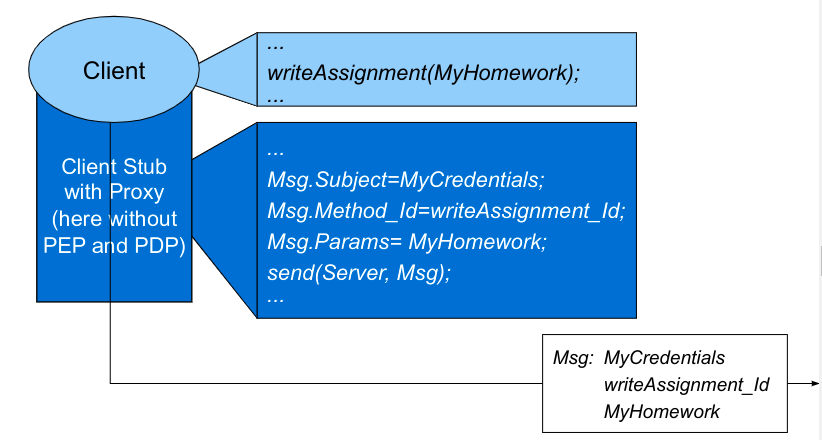
\includegraphics[width=.9\linewidth]{Assets/Systemsicherheit-cobra-1.png}

        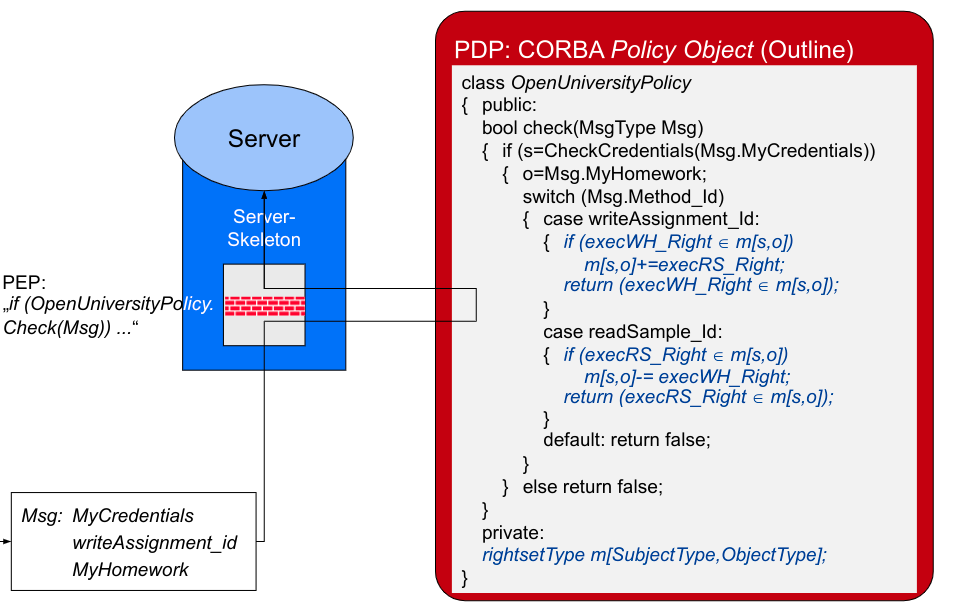
\includegraphics[width=.9\linewidth]{Assets/Systemsicherheit-cobra-2.png}
    \end{multicols*}

    \subsubsection{Kerberos}
    Distributed Authentication and Authorization Architecture with closed user groups( $\rightarrow$ static sets of subjects)
    \begin{itemize*}
        \item Distributed system run by single organization
        \item Workstations and Servers
        \item 2 Kerberos servers
        \begin{itemize*}
            \item Authentication Server (AS)
            \item Authorization Server (TGS)
        \end{itemize*}
        \item Authentication Server (AS)
        \begin{itemize*}
            \item Authenticates users; Based on key shared between user and AS. Result: authenticator (electronic ID card)
            \item Authorizes use of TGS. Based on key shared between AS and TGS. Result: ticket (capability) for TGS
        \end{itemize*}
        \item Ticket Granting Server (TGS): Issues tickets for all servers
        \begin{itemize*}
            \item Based on key shared between TGS and respective server
            \item Result: ticket(s) for server(s)
        \end{itemize*}
        \item Kerberos database
        \begin{itemize*}
            \item Contains for each user and server a mapping $\langle user, server\rangle\rightarrow$ authentication key
            \item Used by AS
            \item Is multiply replicated (availability, scalability)
        \end{itemize*}
    \end{itemize*}

    Typical Use Case
    \begin{enumerate*}
        \item Authentication, then request for TGS ticket
        \item Authenticator, TGS-Ticket
        \item Request for further server tickets
        \item Server tickets
        \item Service request: Servers decide based on
    \end{enumerate*}

    \paragraph{Inside Kerberos Tickets}
    \begin{itemize*}
        \item Tickets issued by Ticket Granting Server
        \item Specify right of one client to use one server (capability)
        \item Limited lifetime (to make cryptographic attacks difficult)
        \begin{itemize*}
            \item balance between secure and convenient
            \item Short: inconvenient but more secure (if stolen soon expires)
            \item Long: insecure but more convenient (no frequent renewal)
        \end{itemize*}
        \item Can be used multiply while valid
        \item Are sealed by TGS with key of server
    \end{itemize*}

    %$T_{Client/Server}=\{Client, Server, Client.NetworkAddress, Timestamp, Lifetime, SessionKey_{Client/Server}\}_{KTGS/Server}$

    Provisions against Misuse
    \begin{itemize*}
        \item Tampering by client to fabricate rights for different server $\rightarrow$ guarantee of integrity by MAC using $K_{TGS/Server}$
        \item Use by third party intercepting ticket $\rightarrow$ personalization by Name and network address of client together with Limited lifetime \&Authenticator of client
    \end{itemize*}

    Authenticators
    \begin{itemize*}
        \item Proof of identity of client to server
        \item Created using $SessionKey_{Client/Server}$
        \begin{itemize*}
            \item[$\rightarrow$] can be created and checked only by
            \item Client (without help by AS, client knows session key )
            \item Server
            \item TGS (trusted)
        \end{itemize*}
        \item Can be used exactly once $\rightarrow$ prevent replay attacks by checking freshness
    \end{itemize*}

    %$A_{Client}=\{Client, Client.NetworkAddress, Timestamp\}_{SessionKey_{Client/Server}}$

    \paragraph{Kerberos Login}
    %The Complete Process 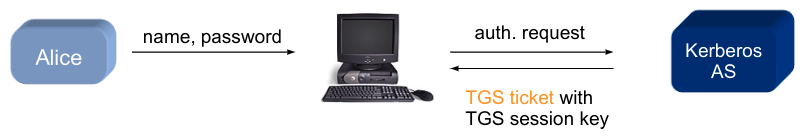
\includegraphics[width=\linewidth]{Assets/Systemsicherheit-kerberos-login.png}
    %Single Steps:
    \begin{enumerate*}
        \item Alice tells her name
        \item Alice’s workstation requests authentication
        \item The AS
        \begin{itemize*}
            \item Create fresh timestamp
            \item Create session key for Alice communication with the TGS % $SessionKey_{Alice/TGS}$
            \item Create Alice ticket for TGS and encrypt it with $K_{AS/TGS}$ %(so Alice cannot modify it): $Ticket_{Alice/TGS}=\{Alice, TGS, \dots , SessionKey_{Alice/TGS}\}_{K_{AS/TGS}}$
            \item Encrypts everything with $K_{Alice/AS}$ (only Alice can read the session key and the TGS-Ticket) %$\{TGS, Timestamp , SessionKey_{Alice/TGS}, Ticket_{Alice/TGS}\}_{K_{Alice/AS}}$
        \end{itemize*}
        \item Alice’s workstation
        \begin{itemize*}
            \item $TGS, Timestamp, SessionKey_{Alice/TGS} , Ticket_{Alice/TGS}$
            \item Requests Alice’s password
            \item Get $K_{Alice/AS}$ from password using cryptographic hash
            \item Uses it to decrypt above message from AS
        \end{itemize*}
    \end{enumerate*}
    \begin{itemize*}
        \item Result: Alice’s workstation has
        \begin{itemize*}
            \item Session key for TGS session: $SessionKey_{Alice/TGS}$
            \item Ticket for TGS: $Ticket_{Alice/TGS}$
            \item The means to create an authenticator
        \end{itemize*}
    \end{itemize*}

    \paragraph{Using a Server}
    Authentication (bidirectional)
    \begin{enumerate*}
        \item Authentication of Client (to server)
        \begin{itemize*}
            \item (Assumption) Alice has session key
            \item (Assumption) Alice has server ticket
        \end{itemize*}
        \begin{enumerate*}
            \item Alice assembles authenticator $A_{Alice}$ %=\{Alice,Alice\_network\_address,timestamp\}_{SessionKey_{Alice/Server}}$ Only Alice can do that, because only she knows $SessionKey_{Alice/Server}$
            \item Alice sends $Ticket_{Alice/Server}, A_{Alice}$ to Server
            \item Server decrypts ticket and thus gets session key; thus it can decrypt $A_{Alice}$ and check
            \begin{itemize*}
                \item Freshness
                \item Compliance of names in ticket and authenticator
                \item Origin of message and network address in authenticator
            \end{itemize*}
        \end{enumerate*}
        \item Authentication of Servers (to client)
        \begin{itemize*}
            \item send $\{Timestamp+1\}_{SessionKey_{Alice/Server}}$ to Alice
            \item only by principal that knows $SessionKey_{Alice/Server}$
            \item only by server that can extract the session key from the ticket %$Ticket_{Alice/Server}=\{Alice,Server ,\dots , SessionKey_{Alice/Server}\}_{K_{TGS/Server}}$
        \end{itemize*}
    \end{enumerate*}

    Getting a Ticket for a Server
    \begin{itemize*}
        \item Are valid for a pair $\langle client, server\rangle$
        \item Are issued (but for TGS-Ticket itself) only by TGS
        \item Ticket request to TGS: $(server, TGS_{ticket}, authenticator)$
    \end{itemize*}

    TGS:
    \begin{itemize*}
        \item Checks $Ticket_{Client/TGS}$ and $authenticator$
        \item Generates $SessionKey_{Client/Server}$ for client \& server
        \item Generates $Ticket_{Client/Server}$
        \item Encrypts both using shared session key $\{Server,$ $SessionKey_{Client/Server},Ticket_{Client/Server}\}_{SessionKey_{Client/TGS}}$
    \end{itemize*}

\end{multicols}

\newpage

\begin{multicols*}{3}

    \subsubsection{Identity-based access control models (IBAC)}
    \begin{itemize*}
        \item ACF: $f_{ABAC}:S\times O\times OP\rightarrow\{true,false\}$ 
        \item ACM: $m:S\times O \rightarrow 2^{OP}$ so $\forall s\in S,\forall o\in O:op\in m(s,o)\Leftrightarrow f(s,o,op)$.
    \end{itemize*}    

    \subsubsection{HRU (Harrison-Ruzzo-Ullman) Safety}
    iff, beginning with q, there is no sequence of commands that enters r in an ACM cell where it did not exist in q

    \subsubsection{TAM Security Model $\langle Q,\sum,\delta,q_0 ,T,R\rangle$}
    \begin{itemize*}
        \item $Q= 2^S\times 2^O\times TYPE\times M$ where $S$ and $O$ are subjects set and objects set as in HRU, where $S\subseteq O$, $TYPE=\{type|type:O\rightarrow T\}$ is a set of possible type functions, $M$ is the set of possible $ACMs$ as in HRU,
        \item $\sum=OP\times X$ is the input alphabet where $OP$ is a set of operations as in HRU, $X=O^k$ is a set of $k$-dim. vectors of arguments of these operations,
        \item $\delta:Q\times\sum\rightarrow Q$ is the state transition function,
        \item $q_0\in Q$ is the initial state,
        \item $T$ is a static (finite) set of types,
        \item $R$ is a (finite) set of access rights.
    \end{itemize*}

    \subsubsection{Theorem 5}
    Safety of a ternary, acyclic, monotonous TAM model (TAMTAM) is decidable in polynomial time

    \subsubsection{Role-based access control models (RBAC)}
    $RBAC_0=\langle U,R,P,S,UA,PA,user,roles\rangle$ where
    \begin{itemize*}
        \item U is a set of user identifiers,
        \item R is a set of role identifiers,
        \item P is a set of permission identifiers,
        \item S is a set of session identifiers,
        \item $UA\subseteq U\times R$ is a many-to-many user-role-relation,
        \item $PA\subseteq P\times R$ is a m:m permission-role-relation,
        \item $user:S\rightarrow U$ function mapping sessions to users,
        \item $roles:S\rightarrow 2^R$ function mapping sessions to roles
    \end{itemize*}
    \begin{itemize*}
        \item $RBAC_1 = RBAC_0 + hierarchies$
        \item $RBAC_2 = RBAC_0 + constraints$
        \item $RBAC_3 = RBAC_0 + RBAC_1 + RBAC_2$
    \end{itemize*}
    \begin{itemize*}
        \item \textbf{Separation of duty} mutually exclusive roles
        \item \textbf{Quantitative constraints} max. number of use
        \item \textbf{Temporal constraints} time/date/week/\dots
    \end{itemize*}
    \begin{itemize*}
        \item $RBAC_1: \langle U,R,P,S,UA,PA,user,roles,RH\rangle$
        \item $RBAC_2: \langle U,R,P,S,UA,PA,user,roles,RE\rangle$
        \item $RBAC_3: \langle U,R,P,S,UA,PA,user,roles,RH,RE\rangle$
        \item $RH\subseteq R\times R$ is a partial order of hierarchy
        \item $RE$ logical expressions over the other model components
    \end{itemize*}

    \subsubsection{Attribute-based access control models (ABAC)}
    Model $\langle S,O,AS,AO,attS,attO,OP,AAR\rangle$ where
    \begin{itemize*}
        \item $S,O$ are subject/object identifiers,
        \item $A_S=V_S^1 \times\dots \times V_S^n$ is a set of subject attributes,
        \item $A_O=V_O^1\times\dots \times V_O^m$ set of object attributes,
        \item $att_S:S\rightarrow A_S$ subject attribute assignment func.,
        \item $att_O:O\rightarrow A_O$ object attribute assignment function,
        \item $OP$ is a set of operation identifiers,
        \item $AAR\subseteq \Phi\times OP$ is the authorization relation.
    \end{itemize*}

    \subsubsection{Denning Security Model}
    a tuple $\langle S,O,L,cl,\bigoplus\rangle$ where
    \begin{itemize*}
        \item $L=\langle C,\leq\rangle$ is a lattice where C is a set of classes, $\leq$ is a dominance relation
        \item $cl:S\cup O\rightarrow C$ is a classification function,
        \item $\bigoplus:C\times C\rightarrow C$ is a reclassification function.
    \end{itemize*}

    \subsubsection{BLP Security Model}
    automaton $\langle S,O,L,Q,\sum,\sigma,q_0,R\rangle$ where
    \begin{itemize*}
        \item S and O are (static) subject and object sets,
        \item $L=\langle C,\leq\rangle$ is a (static) lattice consisting of classes set C, the dominance relation $\leq$,
        \item $Q=M\times CL$ is the state space where
        \begin{itemize*}
            \item $M=\{m|m:S\times O\rightarrow 2^R\}$ set of possible ACMs,
            \item $CL=\{cl|cl:S\cup O\rightarrow C\}$ classify entities in $S\cup O$,
        \end{itemize*}
        \item $\sum$ is the input alphabet,
        \item $\sigma:Q\times \sum\rightarrow Q$ is the state transition function,
        \item $q_0\in Q$ is the initial state,
        \item $R=\{read,write\}$ is the set of access rights.
    \end{itemize*}

    \subsubsection{NI Security Model}
    automaton $\langle Q,\sigma,\delta,\lambda,q_0,D,A,dom,\approx_{NI},Out\rangle$ where
    \begin{itemize*}
        \item Q is the set of (abstract) states,
        \item $\sigma=A$ is the input alphabet, A set of actions,
        \item $\delta:Q\times\sigma\rightarrow Q$ is the state transition function,
        \item $\lambda:Q\times\sigma\rightarrow Out$ is the output function,
        \item $q_0\in Q$ is the initial state,
        \item $D$ is a set of domains,
        \item $dom:A\rightarrow 2^D$ is adomain function that completely defines the set of domains affected by an action,
        \item $\approx_{NI}\subseteq D\times D$ is a non-interference relation,
        \item $Out$ is a set of (abstract) outputs.
    \end{itemize*}
    NI Security Model is also called Goguen/Meseguer-Model.

    \subsubsection{Brewer-Nash Security Model}
    is a deterministic $automaton\langle S,O,Q,\sigma,\delta,q_0,R\rangle$ where
    \begin{itemize*}
        \item $S,O$ sets of subjects (consultants) \& objects (data),
        \item $Q=M\times 2^C\times 2^H$ is the state space where
        \begin{itemize*}
            \item $M=\{m|m:S\times O\rightarrow 2^R\}$ set of possible ACMs,
            \item $C\subseteq O\times O$ is the conflict relation,
            \item $H\subseteq S\times O$ is the history relation,
        \end{itemize*}
        \item $\sigma=OP \times X$ is the input alphabet where
        \begin{itemize*}
            \item $OP=\{read,write\}$ is a set of operations,
            \item $X=S \times O$ arguments of these operations,
        \end{itemize*}
        \item $\delta:Q \times\sigma\rightarrow Q$ is the state transition function,
        \item $q_0\in Q$ is the initial state,
        \item $R=\{read,write\}$ is the set of access rights.
    \end{itemize*}
    
    \subsubsection{Least-Restrictive CW model}
    automaton $\langle S,O,F,\zeta,Q,\sigma,\delta,q_0\rangle$ where
    \begin{itemize*}
        \item S and O are sets of subjects and data objects,
        \item F is the set of client companies,
        \item $\zeta:O\rightarrow F$ mapping each object to its company,
        \item $Q=2^C \times 2^H$ is the state space where
        \begin{itemize*}
            \item $C\subseteq F\times F$ is the conflict relation,
            \item $H=\{Z_e\subseteq F|e\in S\cup O\}$ is the history set,
        \end{itemize*}
        \item $\sigma=OP\times X$ is the input alphabet where
        \begin{itemize*}
            \item $OP=\{read,write\}$ is the set of operations,
            \item $X=S\times O$ arguments of these operations,
        \end{itemize*}
        \item $\delta:Q\times\sigma\rightarrow Q$ is the state transition function,
        \item $q_0\in Q$ is the initial state
    \end{itemize*}

    \subsubsection{Discretionary Access Control (DAC)}
    Individual users specify access rules to objects within their area of responsibility (at their discretion).

    \subsubsection{Mandatory Access Control (MAC)}
    System designers and administrators specify system-wide rules, that apply for all users and cannot be sidestepped.

    \subsubsection{Non-Interference}
    Two domains do not interfere with each other iff no action in one domain can be observed by the other.
    
    \subsubsection{Trusted Computing Base (TCB)}
    The set of functions of an IT system that are necessary and sufficient for implementing its security properties $\rightarrow$ Isolation, Policy Enforcement, Authentication \dots

    \subsubsection{Security Architecture}
    part of a system’s architecture that implement its TCB $\rightarrow$ Security policies, PDP and PEPs, \dots

\end{multicols*}
\end{document}